\documentclass[
a4paper, 
%a5paper,
%10pt,
%11pt,
12pt,
%twoside, % single sided printout
%oneside, % duplex printout (default)
%% binding correction is used to compensate for the paper lost during binding
%% of the document
%BCOR=0.7cm, % binding correction
%nobcorignoretitle, % do not ignore BCOR for title page
%% the following two options only concern the graphics included by the document
%% class
%grayscaletitle, % keep the title in grayscale
grayscalebody, % keep the rest of the document in grayscale
abstract=on,
%% expert options: your mileage may vary
%baseclass=scrreprt % special option to use a different document baseclass
twoside, BCOR10mm, 12pt, DIV13,headinclude, footexclude, final, abstracton, openright
]{ibireprt}


\usepackage[utf8]{inputenc}
%\usepackage[latin1]{inputenc}
\usepackage[T1]{fontenc}
%\usepackage{ngerman}
\usepackage[english]{babel} %ngerman,


%\usepackage{fancyhdr}
%%\pagestyle{fancy}
%%\lhead{\leftmark}
%\fancyhead[OR]{\thepage}% ungerade Seiten, rechts \thepage
%\fancyhead[OL]{\leftmark}% ungerade Seiten, links
%\fancyhead[ER]{\leftmark}% gerade Seiten, rechts
%\fancyhead[EL]{\thepage}% gerade Seiten, links \thepage
%\cfoot{}
%\pagestyle{fancy}
	
\renewcommand{\chaptermark}[1]{\markboth{#1}{}}
\renewcommand{\sectionmark}[1]{\markright{#1}{}}

\setlength{\parindent}{0em}
%\setlength{\parskip}{0mm}
\setcounter{tocdepth}{1}
\setcounter{secnumdepth}{2}
%\linespread{1.15}

\usepackage{quotchap}
\usepackage{nccmath}

\usepackage{microtype}

\usepackage{qtxmath,tgtermes}
\usepackage[scaled=.90]{helvet}
\usepackage{courier}

\usepackage{graphicx}
\usepackage{amsmath}
%\usepackage{amsfonts}
\usepackage{amssymb}
\usepackage{tabularx}
%\usepackage[bookmarks,plainpages=false]{hyperref} %colorlinks  ,urlbordercolor={111},linkbordercolor={111},citebordercolor={111}
\usepackage[Algorithmus]{algorithm}
\usepackage{algorithmic}
%\usepackage{tkmath}
\usepackage{exscale}
\usepackage{empheq}
\usepackage{color}
\usepackage{framed}
\usepackage{rotating}
\usepackage{longtable}
\usepackage[hang,small,bf]{caption}
\usepackage{booktabs}
\usepackage{colortbl}
\usepackage[babel,german=quotes]{csquotes}
\usepackage{ntheorem}
\usepackage{blindtext}
%own userpackages
\usepackage{graphicx} 
\usepackage{subcaption}
\usepackage{comment}
\usepackage[numbers]{natbib}


%\mathindent1.5cm
\def\fleq{\@fleqntrue \let\mathindent\@mathmargin \@mathmargin=\leftmargini}
\def\cneq{\@fleqnfalse}


%\setcapindent{0em}

\newenvironment{fshaded}{%
\def\FrameCommand{\fcolorbox{framecolor}{shadecolor}}%
\MakeFramed {\FrameRestore}}%
{\endMakeFramed}

\theoremseparator{:}

\newtheorem{theorem}{Theorem}[chapter]
\newtheorem{lemma}{Lemma}[chapter]
\newtheorem{remark}[theorem]{Bemerkung}
\newtheorem{definition}[theorem]{Definition}
\newtheorem{example}{Beispiel}
%\newtheorem{proof}[theorem]{Beweis}
\newtheorem{corollary}[theorem]{Corollary}

\newenvironment{Theorem}{\goodbreak \definecolor{shadecolor}{rgb}{0.95,0.95,0.95}%
\definecolor{framecolor}{rgb}{0,0,0}%
\begin{fshaded}\begin{theorem}\sl}{\end{theorem} \end{fshaded}}
\newenvironment{Lemma}{\goodbreak \definecolor{shadecolor}{rgb}{0.95,0.95,0.95}%
\definecolor{framecolor}{rgb}{0,0,0}%
\begin{fshaded} \begin{lemma}\sl}{\end{lemma} \end{fshaded}}
\newenvironment{Remark}{\goodbreak \begin{remark}\rm}{\hfill  $\square$\end{remark}}
\newenvironment{Example}{\goodbreak \begin{example}\rm}{\hfill $\square$ \end{example}}
%\newenvironment{Proof}{\goodbreak \begin{proof}\rm}{\hfill $\blacksquare$ \end{proof}}
\newenvironment{Definition}{\goodbreak \definecolor{shadecolor}{rgb}{0.95,0.95,0.95}%
\definecolor{framecolor}{rgb}{0,0,0}%
\begin{fshaded} \begin{definition}\rm}{\hfill  \end{definition} \end{fshaded} }
\newenvironment{Corollary}{\goodbreak \begin{corollary}\rm}{\end{corollary}}

\newenvironment{Proof}[1][Beweis:]{\begin{trivlist}
\item[\hskip \labelsep {\bfseries #1}]}{\hfill $\blacksquare$\end{trivlist}}

\numberwithin{equation}{chapter}
\numberwithin{table}{chapter}
\numberwithin{figure}{chapter}
\numberwithin{algorithm}{chapter}
\numberwithin{example}{chapter}
\numberwithin{example}{chapter}

\def\i{\mbox{\small{\rm i}}}
\def\ti{\mbox{\scriptsize{\rm i}}}
\newcommand{\e}[1]{{\rm e}^{ #1}}
\renewcommand{\mod}{\;{\rm mod}\;}

\newcommand{\zb}[1]{\mbox{\boldmath{${#1}$}}}
\newcommand{\zbs}[1]{\mbox{\boldmath\scriptsize{${#1}$}}}
\newcommand{\zbss}[1]{\mbox{\boldmath\tiny{${#1}$}}}

\newcommand{\adj}{{\ensuremath{\mathsf{H}}}}
\newcommand{\trans}{{\ensuremath{\mathsf{T}}}}


% Keine "Schusterjungen"
\clubpenalty = 10000
% Keine "Hurenkinder"
\widowpenalty = 10000 \displaywidowpenalty = 10000 %\displaywidowpenalty = 10000






% Information for the Titlepage
\author{Johann Strunck}
\title{Deep learning-based grading of HR-pQCT motion artifacts}
%\date{\today}
\date{\today}
\subject{Bachelor thesis}
\professor{Prof.~Dr.-Ing.~Tobias Knopp}
\advisor{Paul Jürß, M.Sc.}







\begin{document}
%\frontmatter
\maketitle
%\mainmatter


\newpage
${}^{}$
\vfill
\noindent
Ich versichere an Eides statt, die vorliegende Arbeit selbstständig und nur unter Benutzung der angegebenen Quellen und Hilfsmittel angefertigt zu haben.\\
\vspace{1.5cm}

\noindent
Hamburg, den ??.??.2010
\thispagestyle{empty}
\newpage
\newpage

\setlength{\parskip}{1.5mm }

%\newpage

%\maketitle



\tableofcontents



\chapter*{Abstract}
In the field of osteoporosis, high-resolution peripheral quantitative computed tomography (HR-pQCT) scans are used to image bone microarchitecture in vivo at peripheral skeletal sites. However, a common issue with these scans is the appearance of motion artifacts in the resulting images. These artifacts can appear due to involuntary movements, such as twitches and spasms, which occur due to the scan lasting between 2 and 3 minutes. Depending on the severity of these artifacts in the resulting image, it might not be suitable for medical use and a rescan is necessary. The decision regarding the severity of the motion artifacts is made by a qualified individual, who assigns a number from 1 to 5 to the image, with 1 representing no motion artifacts and 5 representing severe motion artifacts. However, this process is inherently subjective and the assigned score can vary depending on the reviewer. Studies have shown that operators disagree in up to 30\% of cases, where a rescan might or might not be necessary \citet{Walle2023}. To support the decision of the operators, an approach was taken by \citet{Walle2023} to improve the confidence of the result by using a convolutional neural network. The findings of this approach were replicated, resulting in a worse model. This might be explained by the fact that XtremeCT I scans were used instead of XtremeCT II scans. XtremeCT II scans are less likely to be in the domain of types 3 and 4, which our networks perform the worst on. Subsequently, the impact of training similar networks by adding and changing layers is evaluated. The results demonstrate that introducing skip connections and inception layers to the network may enhance its performance. One network achieved slightly better peak performances and also exhibited more stable results by switching the last convolution layer for a skip layer with two convolution layers. One of the principal challenges the networks faced was the lack of available training data, which resulted in the networks becoming overly reliant on the available data, a phenomenon known as overfitting.  

%TODO: the F1 Score value still needs to be researched 





	\chapter{Introduction}
\section{Computer Tomography}
High-resolution peripheral quantitative computed tomography (HR-pQCT) is a specialised non-invasive imaging technique that provides detailed and accurate three-dimensional images of bone and tissue micro-architecture of the radius and tibia. This advanced imaging technique offers several distinct advantages, including the ability to provide high-resolution images that allow a thorough assessment of the scanned bone micro-architecture. It also offers precise measurement of Bone Mineral Density (BMD) and geometric parameters such as trabecular thickness and cortical thickness. HR-pQCT has applications in both clinical and research settings, enabling the formulation of more informed decisions about patient management and treatment strategies. It can provide insight into the risk of fracture occurrence.
HR-pQCT is a low-radiation-dose method with an effective radiation dose at the distal radius and tibia of 3-5 \textmu Sv, depending on the scanner generation. Sv is a unit intended to measure the stochastic health risk of ionising radiation. One Sv of ionising radiation exposure results in a 5.5 \% probability of developing fatal cancer. When compared to other common medical imaging techniques, such as chest X-rays with 100 \textmu Sv or hip CT scans with 2000-3000 \textmu Sv, the radiation dose of a HR-pQCT scan is significantly less. This technique is used in the field of osteoporosis. Osteoporosis results in bones becoming weak and brittle, to the extent that even a fall or mild stresses such as bending over or coughing can cause a fracture. Individual studies have demonstrated that HR-pQCT variables can predict incident fractures in postmenopausal women and older men, suggesting that the assessment of cortical and trabecular bone microarchitecture by HR-pQCT could improve overall fracture prediction. 

%There are still no widespread use of HR-pQCT since there is just a small number of devices installed (fewer than 100 in mid 2020) \cite{Bergh2021}.


It is essential that patients remain still during the scan to avoid motion artefacts. This can be challenging for certain patient populations, such as children or individuals with limited mobility. The XtremCT I (Scanco media AG), the device that generated the data used in this thesis, is susceptible to patient movement, as it takes approximately two to three minutes for a scan, which makes it challenging for patients to maintain the selected extremity in a fixed position for such a prolonged period. This is also a concern when the extremity is held in place by a cast.

In the event that the motion artifact is of a sufficiently severe nature, the scan must be repeated. In order to determine the severity of the scan, \citet{Whittier2020} introduced a scale from 1 (no visible motion artifacts) to 5 (significant horizontal streaks) to grade the severity of motion in scans. In clinical studies, it is commonly implemented that scans with a grading of 4 or 5 cannot be used, therefore a rescan is necessary. Nevertheless, even with the implementation of a standardised scoring system, the assessment of motion remains subjective. Operator agreement has been shown to remain only moderate, even with intensive training. Studies have demonstrated that operators disagree in up to 30 \% of cases, as cited in  \citep{Walle2023}. Consequently, there is a clear need for the development of an objective and standardised method for the grading process. Papers such as \citet{Walle2023} and \citet{Sode2011} have attempted to identify an appropriate method for objective grading of motion artifacts, with some success.
%CT
%Computer tomography(CT) is a three dimensional radiographic imaging technique, to obtain detailed internal images of the body, which is commonly used in the field of radiology.The formation process begins with the acquisition of sequential radiographic projections captured over a range of angular positions around the object of interest. The cross sectional field of view is reconstructed using established computational techniques based on the radon projection theory\cite{article}. Similar to simple radiography, the reconstructed image’s intensity values represent the local radiographic attenuation: a material property related to the object’s electron density (atomic number and mass density). The contrast between soft and mineralized tissue in CT is high, due to the relative electron-dense inorganic component (calcium hydroxyapatite) of the bone matrix.These principles capture high-resolution images of bone across a range of structural scales. %TODO: das habe ich koppiert (muss unbedingt  umgeschrieben werden )

%Computer Tomography(CT) is a three dimensional imaging technique which is commonly used in the field of radiology  to obtain internal images of the body. This technique uses a emitter of x-rays which rotates around the specified body part, the rays are then captured by a receiver that measures the beams attenuation. There is a high contrast between the soft and mineralized tissue  due to the electron-dense bone matrix. Afterwards the radon transform can be applied to the collected values from the scan to generate a high resolution three dimensional image of the internal body structure \cite{Burghardt2011}.

%HR-pQCT
%HR-pQCT is a  dedicated extremity imaging system developed to image bone micro architecture in vivo at peripheral skeletal sites \cite{Bergh2021}. This imaging method gives information on the bone structure and mineral density in bones like radius and tibia. This information allows the estimation of the bone strength and ability to resist fracture. The extraction of this information is possible due to the high resolution of HR-pQCT.%TODO: how does it achieve the high resolution 



 
\section{Machine Learning}
%In the last few years a tremendous interest in machine learning emerged. Many applications have found a way in our modern society \cite{LeCun2015}. They can be found in applications like speech to text or the recommendations on e-commerce websites.
%With the emerging field of deep learning in computer vision machine learning got more attention. In 2012 the ILSVRC 2012 challenge  was won by the Convolutional Neural Network (CNN) based Network AlexNet outperforming the runner up with 10.8 percentage points lower top-5 error score of 15.3\%. Since then the application of deep learning structures like CNNs have seen rapid growth in fields like medical imaging. Fields including retinopathy screening, skin lesion classification and lymph node metastasis detection already have research showing that deep learning has a great potential in those fields . This holds also true for the research field of radiology there has been studies in fields like lesion detection, classification and segmentation \cite{Yamashita2018}.

%A frequently occurring issue in medical imaging is the lack of training data. In our case we had 500 labeled examples of tibia and radius. If we compare this to the amount of data used in training state of the art networks with datasets like MNIST, CIFAR or ImageNet ranging from many thousand labeled images to over a million examples it's a small fraction. The main reason is that the labeling task in medical imaging can just be performed by professionals and therefore the process is costly and just a few people can do it. The data that we use in this paper to compare the different approaches was provided by the osteology department of the Universitätsklinikum Hamburg-Eppendorf. All 500 provided scans where generated by the Scanco XtremCT I. To ensure the correctness of the labels, three doctors labeled the data separate from each other. This allowed the values of the labels to be generalized reducing the subjective influence of the single person. To get a stable network with a somewhat high accuracy we have to find a way to augment the data so that we don't run into problems like overfitting or poor generalization of the network. This paper will compare different augmentation techniques and their impact on the training of the network given by \cite{Walle2023}. 

%TODO: maybe we should also already talk about the necessity of weighted loss but maybe we should introduce it with walles network 
 
%This paper uses CNNs to train a network for grading motion artifacts. Deep learning techniques, particularly CNNs, have revolutionized medical image analysis. CNNs are a subset of Artificial Neural Networks(ANNs), with each node detecting local features from the input vector, minimizing the parameters in a process called down-sampling, and the subsequent layers combining these features into a fully connected layer.%TODO: rewrite last sentence in own words 

%CNNs excel at tasks such as image segmentation, object detection, and classification. With their ability to automatically learn intricate patterns and features from complex visual data, enabling more accurate and efficient diagnostic processes. %more information necessary 
%Even with the simplistic structure chosen in \cite{Walle2023} the network is reaching a F1 Score of 86.8$\pm$2.8\%, this can lead to the assumption that a more sophisticated network might reach better results. This paper builds on the findings and tries to create a stronger network with state of the art CNN building blocks.  

%This paper tries to replicate the findings of \cite{Walle2023}. To achieve a high accuracy we evaluate which augmentation methods and learning rates are best suited for its training, afterwards modified network structures are  compared and their results are interpreted. 

%TODO: can defenetly be longer 


%machine learning 
In recent years, machine learning has emerged as a prominent field within the research domain, largely due to its adaptable nature. It is a branch of artificial intelligence and computer science that focuses on algorithms capable of learning from data and generalising for unseen data. One approach to machine learning is supervised learning, which involves training an algorithm on labelled data. This entails providing the algorithm with pairs of input and output values. The objective of training the algorithm to perform well on labelled data is to enable it to generalise its performance to unseen data. Consequently, the data is typically divided into a test and training set. This reduces the amount of training data available, but it allows for an understanding of how the network might perform on unseen data.
 
%A machine learning algorithm operates by processing data to identify patterns and connections. It learns from the data through a training process, adjusting its internal parameters to minimize a measure called "loss". The loss quantifies the difference between the algorithm's predictions and the actual outcomes in the training data. The algorithm iterative refines its parameters to reduce this loss, making its predictions more accurate. Once trained, the algorithm can apply its learning to new, unseen data, aiming to make predictions or classifications with minimized error based on its learned patterns.

\begin{figure}[h]
	\centering
	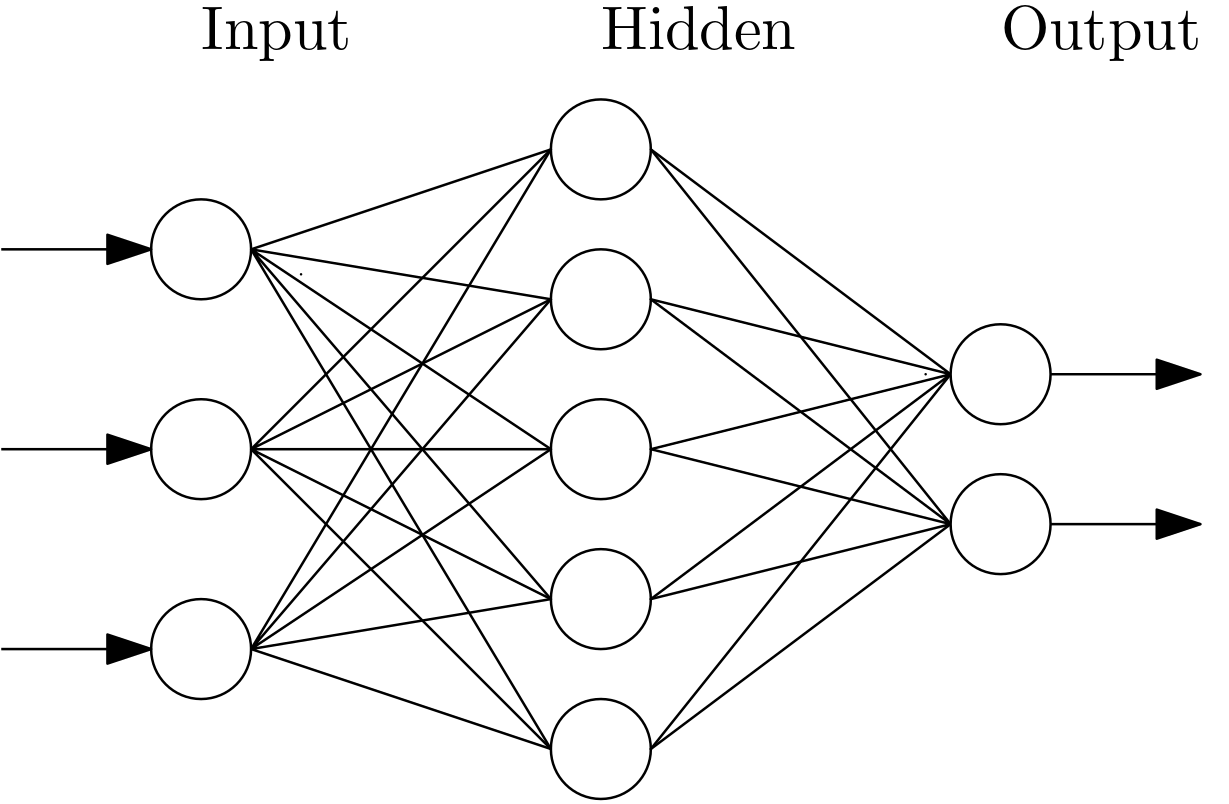
\includegraphics[width =0.4 \textwidth]{ANN_network.png}%
	\caption{Artificial neural network}
	\label{fig:ANN_network}
\end{figure}

Artificial neural networks represent one branch of machine learning. A neural network is composed of an input and output layer, as well as one or multiple hidden layers. Each layer contains nodes, with each node being connected to all nodes in the following layer. The hidden and output nodes calculate the sum of all input values, $x_i$, multiplied with their corresponding weight, $w_i$. Such layers are also employed in more complex networks and are usually denoted as dense or fully connected layers. Each node typically contains a bias, b, which is added to the weighted sum of the input values. This is then fed through a nonlinear activation function. 

% Each hidden layer consists of interconnected nodes, also called neurons, where each output neuron is usually connected to every input. This feature enables the network to make high-level decisions based on the learned features. Each connection between nodes has an associated weight. To calculate the output of a FC layer the weighted sum for every single neuron is calculated. Most of the time a bias is added to the sum. Afterwards, an activation function is applied. 

\begin{align}
	y(x)=acitvaion((\sum_{i=1}^{n}w_i\cdot x_i)+b)
\end{align}


%https://builtin.com/sites/www.builtin.com/files/styles/ckeditor_optimize/public/inline-images/3_fully-connected-layer_0.jpg

\subsection{Activation Function}
%Activation functions 
This type of function is employed in networks to enable the representation of more complex functions. They are also utilised to map the input into the requisite number range, such as a value between 0 and 1 or 1 and -1. The selection of the activation function has a significant impact on the capability and performance of the neural network. It can facilitate the identification of intricate patterns and even accelerate the learning process \citep{Khan2020}.  


\begin{align}
	\sigma (x)= \frac{1}{1+e^{-x}}
\end{align}

The ReLU function offers significant advantages over the sigmoidal function in a neural network. The main advantage is that the ReLU function is highly efficient in terms of computation time. For positive inputs, the ReLU function has a constant gradient of 1, whereas a sigmoid function has a gradient that rapidly converges to zero. This property makes neural networks with a sigmoid activation function slower to train. This phenomenon is also known as the vanishing gradient problem. The sigmoid function maps a large input space between 0 and 1. Consequently, a substantial alteration in input may result in a relatively minor alteration in output, which in turn leads to a reduction in the derivative. This phenomenon impairs the efficiency of parameter updates. 


The ReLU activation function is less susceptible to this problem because the gradient of ReLU is always one for positive x, preventing the learning process from being slowed down by a vanishing gradient. 


\begin{align}
	ReLU(x) = \max(x,0)
\end{align}

However, the zero gradient can still cause the vanishing gradient problem.

This can be compensated for by adding a smaller linear term in x to give the ReLU function a non-zero gradient at all points. This is solved in the implementation of ELU by adding $\alpha \ (e^x-1)$ for all values less than zero. Therefore the slope of ELU is always greater than 0 and tends to zero for $x \rightarrow - \infty$.


\begin{align}
	ELU(x) = 
	\begin{dcases}
		x \text{, if } x \geq 0 \\
		\alpha \ (e^x-1) \text{, otherwise}
	\end{dcases}
\end{align}

There are numerous other activation functions that have been proposed, but ReLU or ELU is arguably the most commonly used. In fact, \citet{Mishkin2017} even recommends using ELU non-linearity without batch normalisation or ReLU with it.
%ReLU

In the context of training a multiclass network where only one or a few classes are to be classified, the softmax function can be employed as the last layer activation function. The softmax function utilises the exponential function, $e^x$, to scale the values, thereby facilitating the differentiation between singular values and enabling a more discernible distinction. Of note is the fact that the sum of all outputs from the softmax function is equal to one. This is a valuable attribute, as the outputs can be converted directly to percentages. This can be interpreted as the probability of an image showing a particular class. Mathematically, this means that the output O$_j$ of a network is treated as a probability P.

\begin{align}
	O_j = P \ (c= j | input)
\end{align}

This requires: 

\begin{align}
	O_j > 0 
	\quad and \quad
	\sum_{j=1}^{N} O_j = 1 
\end{align}

 
To enforce this stochastic constraint \citet{Bridle1990} proposes a normalized exponential output. The input values, $I_x$, are unconstrained and represent the output values of the previous layer in the context of a last layer activation function. 

\begin{align}
	O_j = \frac{e^{I_j}}{\sum_{k}^{} e^{I_k}} 	
\end{align}

Another last layer activation function is the sigmoid activation function which is commonly used for binary classification.
The graph of the sigmoid function is a S shaped curve that is 0.5 for $\sigma(0)$. It converges to 1 for x $\rightarrow \infty$ and 0 for x $\rightarrow -\infty$. This ensures that the values range between 0 and 1 and also gives the possibility to interpret the output as a probability. 


\subsection{Loss}


To assess the performance of a network on data, we utilise a loss function that quantifies the deviation of the network's output, denoted by $\hat{y_i}$, to the ground truth, represented by $y_i$, across a set of $N$ elements. In machine learning, these functions are categorised based on the task they are employed for. The majority of them can be applied to either classification or regression tasks. One of the earliest loss functions in machine learning is the $L^2$ (also known as Mean Squared Error) loss, which is typically used for regression tasks. This function quantifies the magnitude of the error between the prediction and actual output of a network. The squaring of the error results in a higher penalty for higher deviations from the target value. 
\begin{align}
	loss(y,\hat{y})=\frac{1}{N}\cdot \sum^{N}_{i=1}(y_i-\hat{y_i})^2
\end{align}
%crossentropy loss 

The majority of object detectors employ cross-entropy-based loss functions for classification purposes. This function represents the most fundamental loss function for classification tasks. 

\begin{align}
	loss(y,\hat{y}) = - \frac{1}{N} \cdot \sum_{i=1}^{N}y_i \cdot log(\hat{y}_i)
\end{align}

%There are many functions derived from the cross entropy loss like Kullback-Leibler divergence and Jensen Shannon divergence. \cite{Tian2022} shows that in a classification task, that cross entropy loss is equivalent to the other models as long as the ground truth is known. 
%Since cross entropy loss does not involve the real distribution entropy and gets more stable results, it will be used in this thesis. 

One of the most common issues encountered in classification tasks is the imbalance of data. This can result in the model being biased and performing poorly on smaller classes. To address this issue, weighted loss can be employed. This function is a modification of standard loss, which assigns higher weights to minor classes. The weights are calculated based on the ratio between the total number of samples and the number of samples in the given class. 

\begin{align}
	w_i = \frac{total\_samples}{number\_samples\_in\_class\_i \cdot num\_classes}
\end{align}

Subsequently, the weights are applied to the cross-entropy loss, which is also known as the weighted cross-entropy loss. 

\begin{align}
	loss(y,\hat{y})= -	\frac{1}{N}\cdot \sum_{i=1}^{N} w_i \cdot y_i \cdot log(\hat{y}_i)
\end{align}

The application of weights to the loss function enhances the model's sensitivity to the misclassification of underrepresented classes. This directs the network towards a direction that also improves the performance of underrepresented classes.

Weighted loss can also be applied to a single-class classification model. This is because there is a binary cross-entropy loss function.

\begin{align}
	loss(y,\hat{y})=\frac{1}{N}\cdot\sum_{i=1}^{N} -w_i \cdot (y_i \cdot log(\sigma(\hat{y_i}))+(1-y_i)\cdot log(1-\sigma(\hat{y_i})) )
\end{align}

%TODO: maybe check if we can get a transition or change the start of optimizers

\section{Optimizer}
%optimizers
In order to optimise the performance of the network on the given data, the network parameters must be adapted in such a way that the loss on the training set is reduced. This also has the effect of increasing the network's accuracy on the training data. The process of refining the parameters is carried out by a so-called optimiser. There are various different optimisation algorithms, including stochastic gradient descent, RMSprop, Momentum or Adam. These algorithms differ in their approach to calculating and applying parameter updates based on the gradients of the loss function with respect to the model parameters (weight and biases) during training. The optimiser seeks to identify the optimal set of parameters by iterative updating the parameters in a way that converges the model in a direction of decreasing loss.

Gradient descent is a widely employed method for optimising a neural network \citep{Ruder2016}.  It is based on the observation that if a function $F$ is differentiable in the vicinity of $a$, $F$ will decrease the fastest if one moves from $a$ in the direction of the negative gradient of $F$ at $a$. There are three distinct variants of gradient descent, distinguished by the extent to which data is employed to calculate the gradient of the loss function. There are three variants of gradient descent: stochastic gradient descent, batch gradient descent and mini-batch gradient descent. 

Mini-batch gradient descent represents a compromise between stochastic gradient descent and batch gradient descent. It is characterised by the use of a small amount of data for calculating the gradient, which results in greater accuracy than stochastic gradient descent. However, it is less efficient than stochastic gradient descent, as it calculates its gradient based on a single example. In contrast, batch gradient descent is faster than mini-batch gradient descent, as it takes all the examples into account. Consequently, batch gradient descent is more accurate than mini-batch gradient descent. Mini batch gradient descent represents a compromise between the other two variants, offering a good balance between computation cost and accuracy. It is the most commonly used gradient descent algorithm.

By calculating the gradient of the function represented by the network, we are able to update its weights. This fits the function to the data, reducing the loss for this particular set. The amount of change to the model during each step can be regulated by the learning rate, denoted by $\eta$. A small learning rate impedes the network's ability to learn effectively, while a large learning rate can result in the network exhibiting divergent behaviour. To ensure that the network learns in a timely manner while avoiding overshooting, it is typical to start with a larger learning rate and then gradually decrease it as the training progresses.
  
%Adam 
Since the advent of gradient descent, there has been a significant advancement in the field of machine learning, with the development of numerous more efficient algorithms. Adaptive Moment Estimation (Adam) \citet{Kingma2014} is a first-order gradient-based optimization technique or learning algorithm that has gained widespread adoption, representing the latest trend in deep learning optimization. Adam is a deep learning strategy that was specifically designed for training deep neural networks. Its primary advantage is its rapid convergence, while still maintaining memory efficiency and a relatively low computational cost compared to other optimization algorithms. 
The algorithm utilises the squared gradients ($v_t$) to scale the learning rate in a manner analogous to RMSprop, and is analogous to momentum in that it employs the moving average of the gradient ($m_t$).


\begin{align}
	& g_t = \nabla_\theta f_t(\theta_{t-1})\\
	& m_t =\beta_1\cdot m_{t-1} + (1- \beta_1)\cdot g_t \\
	& v_t =\beta_2\cdot v_{t-1} + (1- \beta_2)\cdot g_t^2
\end{align}

The first moment (the mean) and the second moment (the uncentered variance) of the gradient are estimated as $m_t$ and $v_t$, respectively. These estimates are used to calculate an individual learning rate for different parameters. The moving averages are initialized as vectors of 0's, which biases the moment estimates towards zero. However, this initialization bias can be counteracted, resulting in bias-corrected estimates, denoted by $\hat{m}_t$ and $\hat{v}_t$.

\begin{align}
	\hat{m}_t =\frac{m_t}{1- \beta_1^t} \\
	\hat{v}_t = \frac{v_t}{1- \beta_2^t}
\end{align}

Those moment estimates can then be used to update the parameters: 

\begin{align}
	\theta_t = \theta_{t-1}-\alpha\cdot\frac{\hat{m}_t}{\sqrt{\hat{v}_t}+\epsilon}
\end{align}

The default settings are as follows: the step size is set to $\alpha = 0.001$, the exponential decay rates for the moment estimates are $\beta_1 = 0.9\ \beta_2 = 0.999$, and $\epsilon =  10^{-10}$. These settings can then be refined to better fit the optimization task.

Although Adam has the capacity to modify its learning rate, there are instances where this is insufficient. \citet{Loshchilov2017}  states that the $L^2$ regularisation approach of Adam is less effective than weight decay, prompting the development of ADAMW. This is a modified version of Adam that separates the weight decay from the gradient-based update. The principal distinction between ADAMW and Adam lies in the formulae employed for calculating the gradient and update parameter.
It is argued that the L2 regularisation approach of Adam is not as efficacious as weight decay, and therefore ADAMW was developed as a modified version of Adam. This approach decouples the weight decay from the gradient-based update. The principal distinction between ADAMW and Adam lies in the formulae employed for calculating the gradient and update parameter. 
\begin{align}
	&g_t  = \nabla_\theta f_t(\theta_{t-1})+\lambda\cdot\theta_{t-1}\\
	&\theta_t = \theta_{t-1}-\eta_t (\alpha\cdot\hat{m}_t(\sqrt{\hat{v}_t}+\epsilon)+\lambda\theta_{t-1})
\end{align}  

In this formula, the variable $\eta_t$ represents the schedule multiplier, which can be either fixed or decay. The variable $\lambda$ represents a fixed multiplier. The results of the paper demonstrate a 15\% relative improvement in test error compared to Adam for various image recognition datasets.

%TODO:entscheiden ob der teil drinnen bleibt 
%The use of Adam is typically insufficient to achieve optimal results in the absence of additional gradient noise. In one of the experiments conducted by \cite{Neelakantan2015}, multiple approaches were employed to train a network on the MNIST data set. Each approach was evaluated with and without the addition of Gaussian noise to the test data. The results of this experiment demonstrated that in all of the selected cases, the test accuracy and average test accuracy increased with the introduction of noise, with the exception of one case where the average test accuracy remained unchanged. 

%bis hierhin kontrolliert

\subsection{Convolutional Neural Networks}
%CNN
ANNs are effective for a wide range of tasks, but they are less suitable for image processing or recognition tasks. This is because, as they are only capable of processing arrays as input data, the spatial information contained in an image is lost, as the relationship between neighbouring pixels is removed. Furthermore, the number of parameters required increases quadratically with the size of an image, resulting in a large number of input nodes, which makes the training computationally expensive.A network with a large number of parameters can also be susceptible to overfitting.

Convolutional neural networks (CNNs) are a class of deep learning models that have been specifically designed for processing structured grid-like data, such as images. This is achieved by automatically learning hierarchical patterns and features. CNNs are widely used in computer vision tasks and have revolutionised the field of image recognition, object detection, and image generation. CNNs excel at tasks like image classification, where the network assigns a label or category to an input image. The primary advantage of CNNs over ANNs is the reduced number of parameters required for the networks. Additionally, CNNs are capable of recognizing patterns with spatial hierarchies. 
%Convolutional Layer

The fundamental building blocks of CNNs are convolution layers, which perform convolution operations on input data. These layers apply a set of learnable filters (also called kernels) to the input images by sliding the filter over the data and computing element-wise multiplications and summations to produce feature maps, as illustrated in Figure \ref{fig:fig2}. The purpose of these layers is to detect different features, such as edges, textures, and more complex patterns. As the learned features pass through multiple convolution layers, they become progressively more abstract, enabling the classification of complex structures. Two key hyperparameters that define the convolution operation are size and number of kernels. The former is typically 3 × 3, but sometimes 5 × 5 or 7 × 7. The application of a convolution layer on a matrix shrinks it in size. 

To achieve the desired output size, two parameters, named padding and stride, can be modified to modify the output size. The first possibility is to add padding, which adds a number of zero rows and columns to the input. This increases the resulting output size. During the convolution, the filter slides over the matrix from left to right and from top to bottom. Stride is the second changeable parameter. It defines the step size of the filter. Consequently, it determines the number of elements that the filter moves to the right or bottom per iteration.


\begin{figure}[h]
	\center
	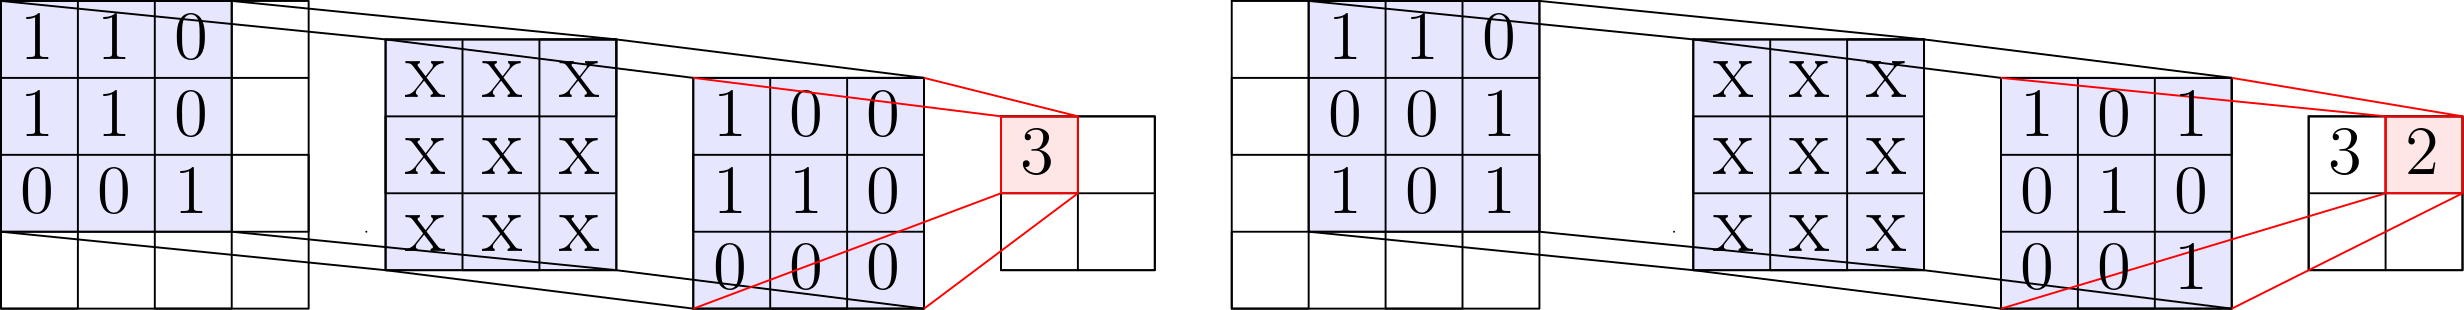
\includegraphics[width = 1 \textwidth]{3x3_conv_layer.png}%
	\caption{Convolutional Layer with Kernel 3x3}
	\label{fig:fig2}
	%https://datascience.stackexchange.com/questions/80436/understanding-how-convolutional-layers-work
\end{figure}

\subsection{Pooling Layer}
%Pooling Layer
The convolution layer is typically followed by a pooling layer. This layer reduces the spatial dimensions of the feature maps while retaining important information. The stride typically matches the field size of the pooling operation, ensuring that no feature of the previous layer is used twice. Max pooling and average pooling are the most common applied pooling operations. In the max pooling operation, the maximum value of the current view is selected, thereby preserving detected features, particularly the most commonly used. The average pooling operation involves calculating the mean value of the values of the current view. During training in back propagation, average pooling provides a more gradual change in gradient compared to max pooling. It also retains information from the original image since average pooling takes the collective information into account, whereas max-pooling results in the loss of at least 75\% of the previous images data. 

\begin{figure}[h]
	\centering
	\begin{minipage}[t]{.45\linewidth}
		\centering
		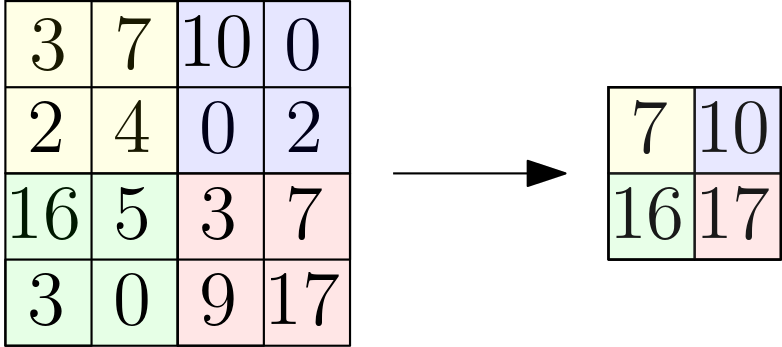
\includegraphics[width = \textwidth]{max_pool.png}%
		\caption{Max Pooling Layer with Kernel 2x2 and Stride 2}
		\label{fig:fig_max_pooling}
		
	\end{minipage}
	\hfill
	\begin{minipage}[t]{.45\linewidth}
		\centering
		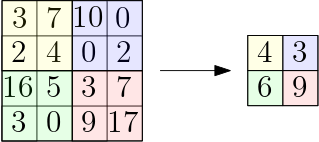
\includegraphics[width = \textwidth]{average_pool.png}%
		\caption{Average Pooling Layer with Kernel 2x2 and Stride 2}
		\label{fig:fig_average_pooling}
	\end{minipage}
	%https://www.baeldung.com/cs/neural-networks-pooling-layers
\end{figure}
\begin{align}
	MaxPooling(X)_{i,j,k} = \max_{m,n}X_{i\cdot s_x + m, j \cdot s_y+n,k}
\end{align}
\begin{align}
	AveragePooling(X)_{i,j,k} =\frac{1}{f_x\cdot f_y}\sum_{m,n} X_{i\cdot s_x + m, j \cdot s_y+n,k}
\end{align}

 X is the input, k is the channel index, $s_x$ and $s_y$ are the stride values in the horizontal and vertical directions, respectively, and the pooling window is defined by the filter size $f_x$ and $f_y$.

Following the application of a number of convolutional and pooling layers, the output is typically flattened. This process enables the subsequent introduction of dense layers, which are used to shape the output to the desired size.



%TODO: make a patr about this it sounds very interresting it pairs well with CBAM most of recent network engineering methods mainly target on three factors depth [19,9,10,5], width [10,22,6,8], and cardinality [7,11], we focus on the other aspect, ‘attention’, 
%to incorporate: global average pulled features are  suboptimal features in order to infer fine channel attention and we suggest to use max-pooled features as well	


\subsection{ImageNet}
The ImageNet Image Large Scale Visual Recognition Challenge (ILSVRC) is an annual competition in the field of computer vision which focuses on object detection and image classification. In the initial challenge, which was held from 2010 to 2017, numerous breakthroughs were observed, with the performance of networks rapidly improving. Following this, the data set was updated, and the challenge continues to the present day. The challenge involves training and evaluating algorithms on the ImageNet data set, which contains millions of labelled images across thousands of categories. Many breakthroughs in deep learning, particularly in convolutional neural networks (CNNs), can be traced back to this challenge.

%AlexNet
%In the history of CNNs AlexNet is a pioneering architecture that played a pivotal role in advancing the field of deep learning and computer vision. \cite{Alzubaidi2021} In 2012 Alex net won the Image Net Large Scale Visual Recognition Challenge(ILSVRC) since it introduced several groundbreaking concepts, including deep architecture with multiple convolution and fully connected layers, ReLU activation functions, dropout for regularization, and GPU acceleration for faster training. Its success highlighted the potential of deep neural networks for image classification tasks. It influenced the design of subsequent CNN architectures and shaped the direction of modern deep learning research.

%network in Network 
%GoogleNet / Inception Module
\subsection{GoogleNet}
GoogleNet (also known as Inception-V1), the winner of the 2014 ILSVRC competition, introduced the inception block into its network, achieving high accuracy with decreased computational cost. In the paper of \citet{Szegedy2015} convolution layers are replaced with small blocks, similar to the idea of substituting each layer with smaller networks. The inception block makes use of the idea that larger filters of size 11x11 or 5x5 can be replaced by a stack of 3x3 filters. The use of smaller filters reduces computational complexity and induces the effect of large-scale filters. The inception block includes filters of size 1x1, 3x3 and 5x5 to capture spatial information at different scales. The split transform and merge concept addresses a problem related to the learning of diverse types of variations present in the same category of images.% look at network in network (NIN) and VGG net



%Since the introduction of Inception-V1 progress has been made. The latest model Inception-V3/V4 was to minimize the computational cost with no effect on the deeper network generation by using asymmetric small-size filters (1x5 and 1x7) rather then large scale filters. Moreover they utilized the bottleneck of a 1x1 convolution layer prior to the large size filters. 

\begin{figure}[h]	
	\centering
	\begin{minipage}[t]{.49\linewidth}
		\centering
		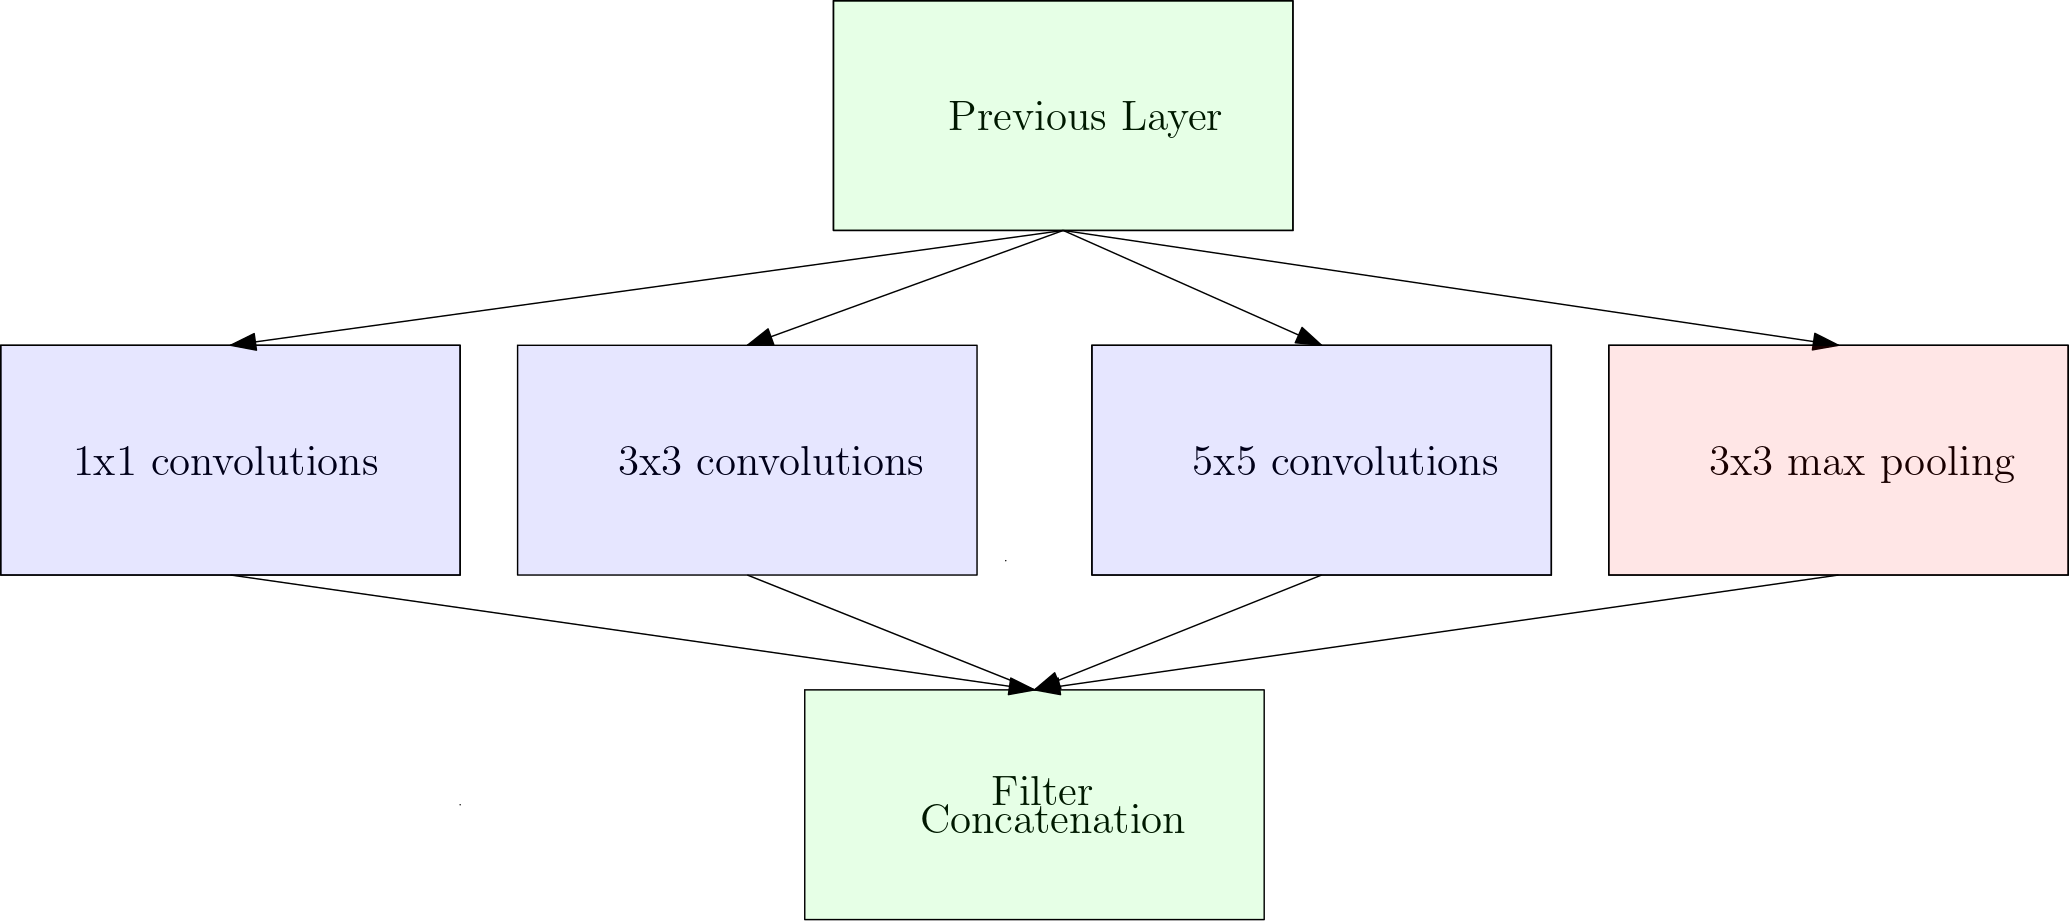
\includegraphics[width = \textwidth]{Inception_modle_naive.png}%
		\caption{Naive Inception Module}
		\label{fig:fig_max_pooling}
		
	\end{minipage}
	\hfill
	\begin{minipage}[t]{.49\linewidth}
		\centering
		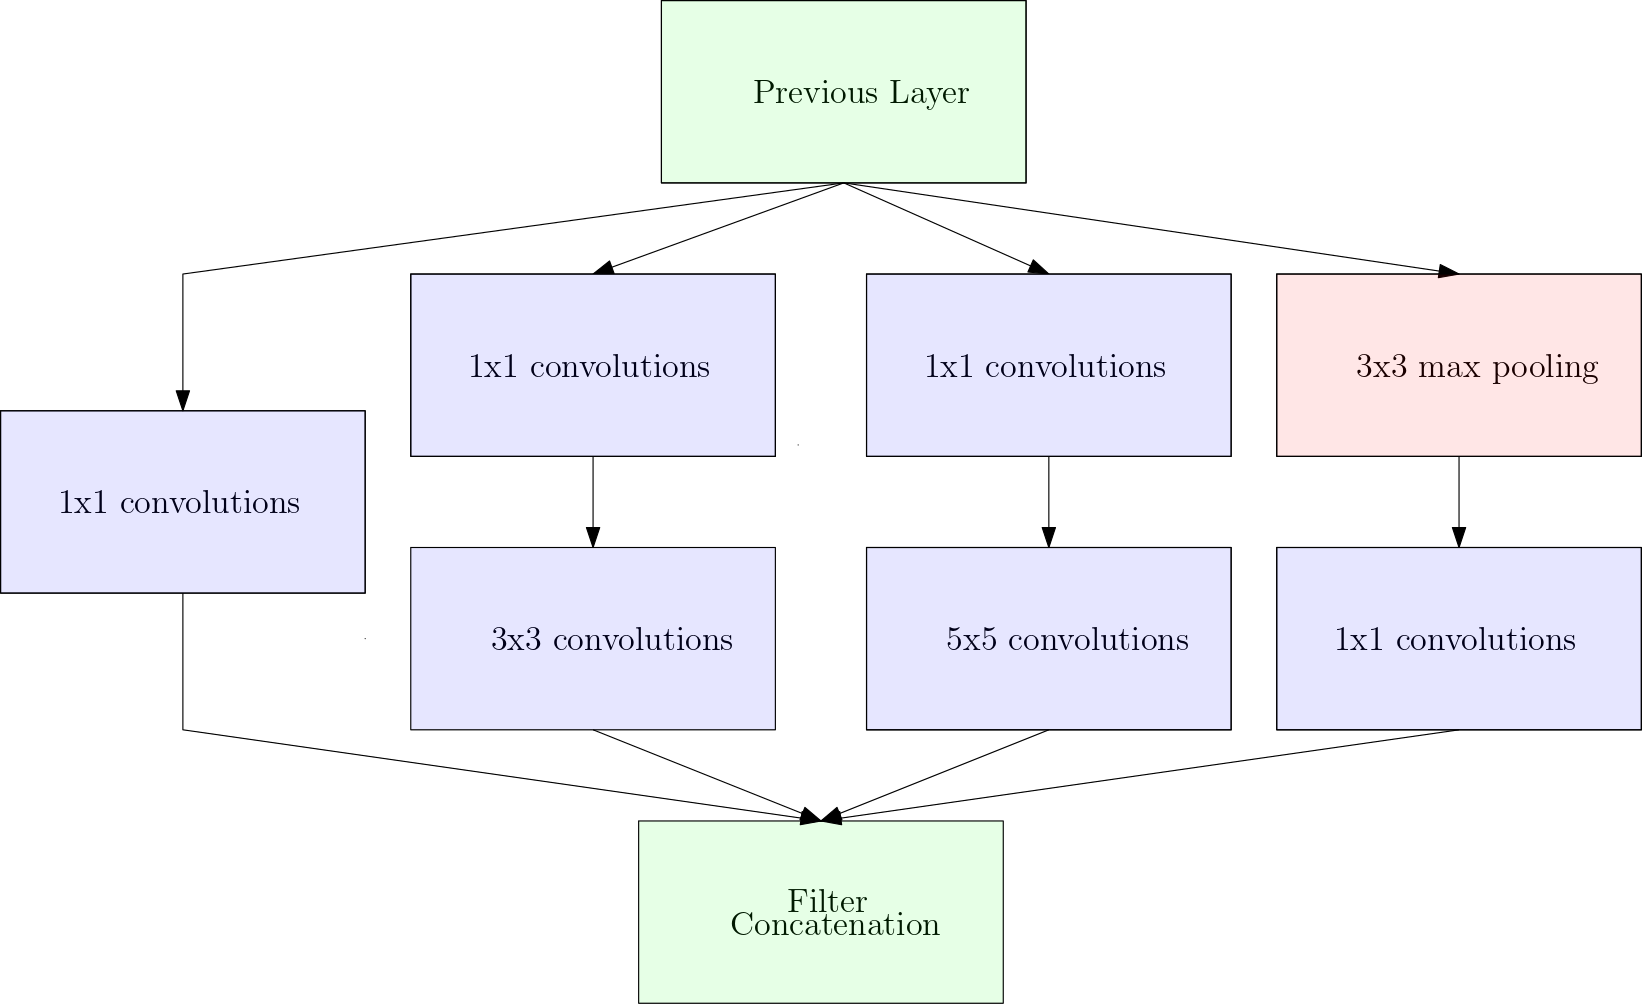
\includegraphics[width = \textwidth]{Inception_modle_reduction.png}%
		\caption{Inception Module With Reduction}
		\label{fig:fig_max_pooling}
		
	\end{minipage}
\end{figure}%


\subsection{ResNet}
%ResNet ILSVRC 2015 
In 2015, \citet{He2016a}  won the ILSVRC competition with their Residual Networks (ResNet). These networks utilise a special component, the shortcut connection, which facilitates the training of deeper networks. The shortcut connection allows the input data of a layer to be connected with the output of that layer, thereby retaining input information. A notable advantage of this connection is that it does not introduce new parameters or computational complexity to the network. As illustrated in \ref{fig:ResNet_block}, it is not uncommon to have more than one convolutional layer between a shortcut connection. Typically, two to three convolutional layers are employed, although more are possible. One convolutional layer is rarely used, as it is akin to using a linear layer, which would not benefit the network.

% usually more than 1 conv layer since it is more equal to a linear layer wich has no significant advantages , usually its 2 or 3 layer but more are possible 

\begin{figure}[h]	
	\center
	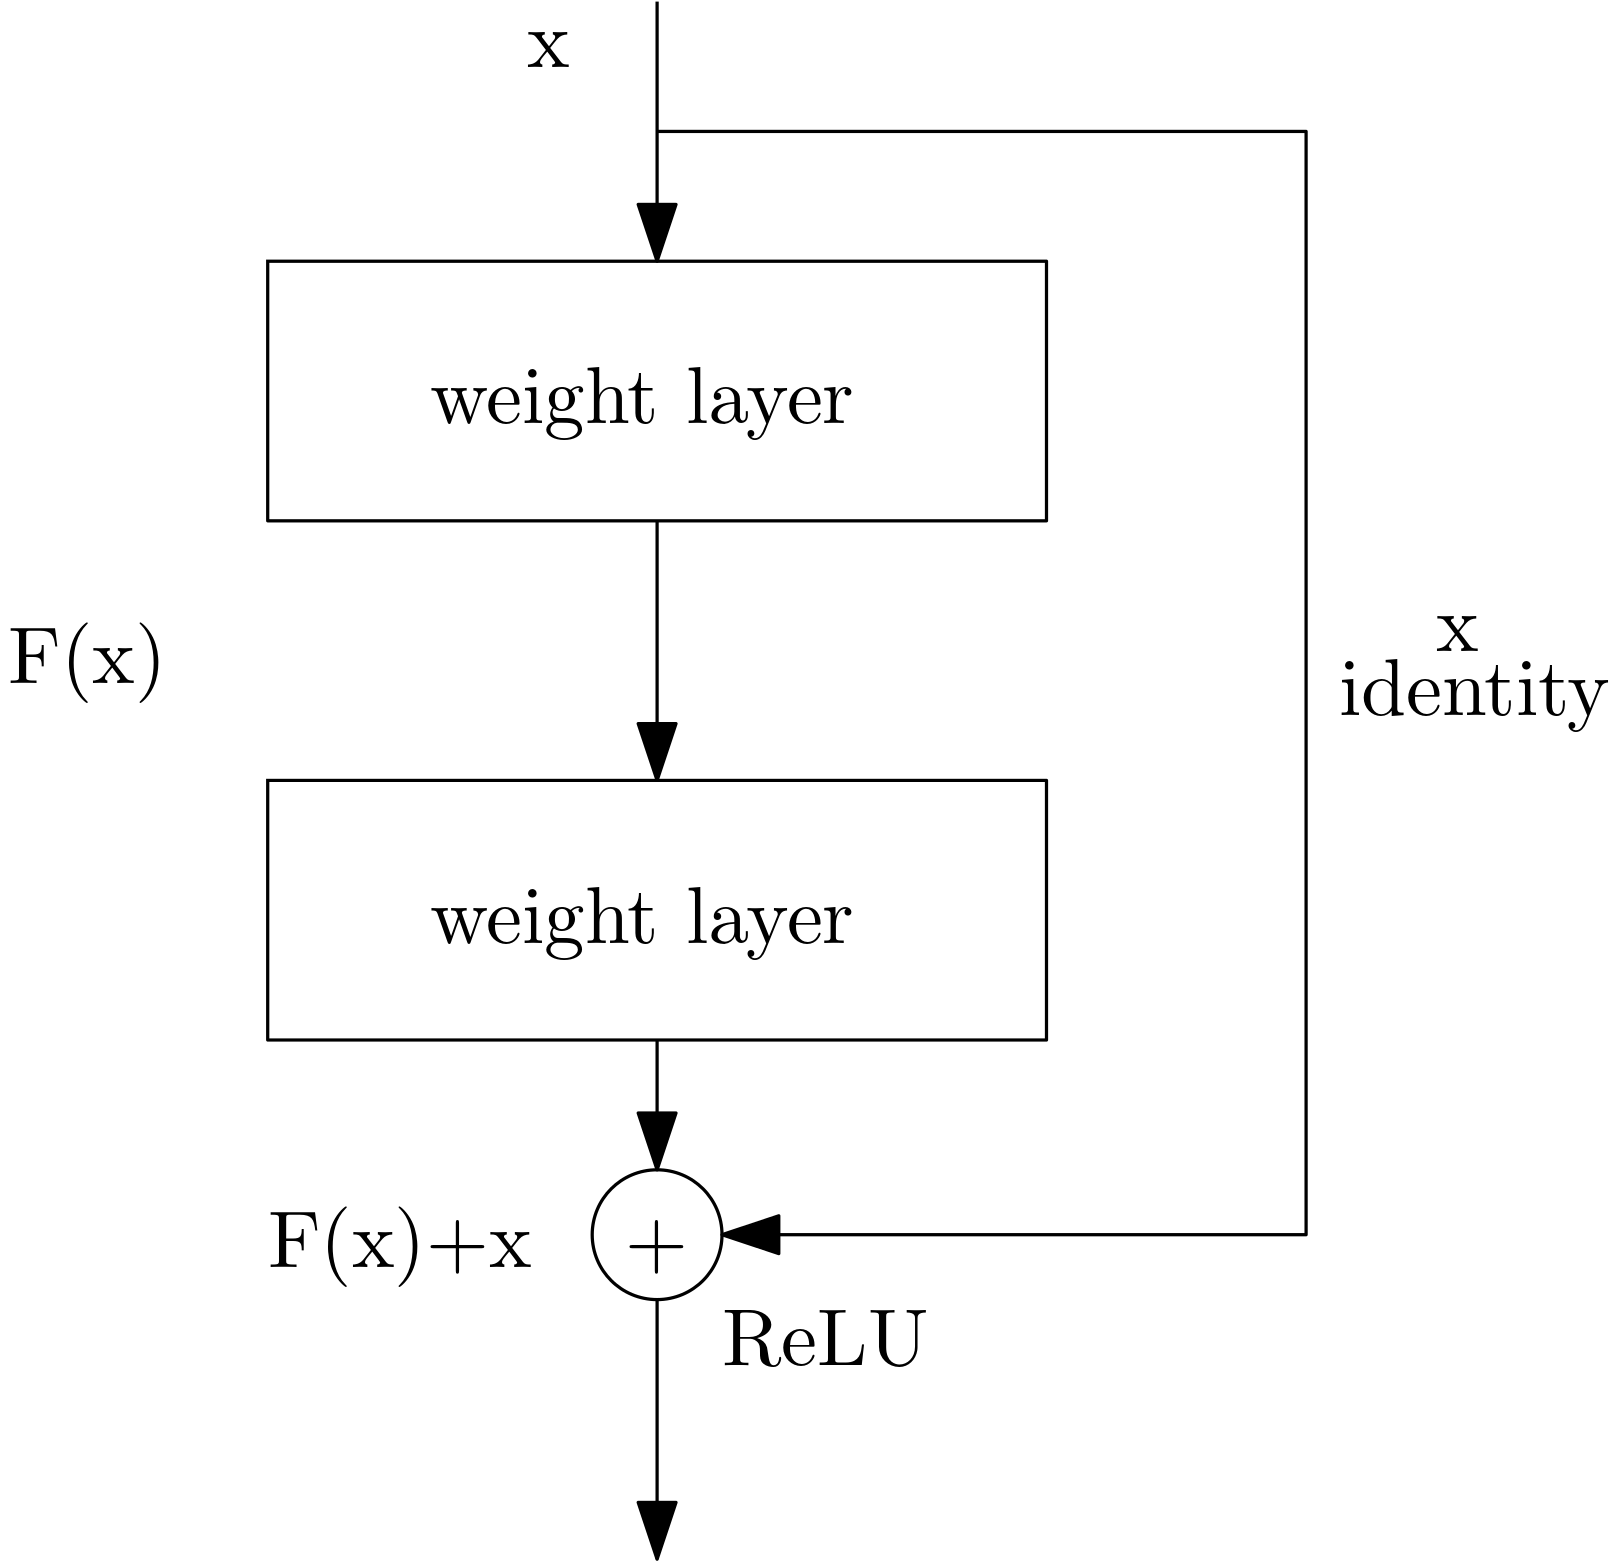
\includegraphics[width = 0.4 \textwidth]{conv_layer_with_skip_connection.png}%
	\caption{Convolutional layers with shortcut connection}
	\label{fig:ResNet_block}
\end{figure}%


\subsection{Existing Network Structure}
\citet{Walle2023} introduces a CNN structure which is trained to classify the severity of motion artefacts in HR-pQCT. The network is trained with images (XtremeCT II, Scanco media AG) from 90 patients. The size of the scans is 512 x 512 x 168 pixels. The training set comprises eight images from each scan, resulting in a database of 3312 images. The training set images are randomly flipped horizontally and vertically. The network structure begins with four alternating convolution and max-pooling layers, followed by another convolution layer. The convolution layers employ leaky ReLU as an activation function, enabling faster learning while avoiding dead neurons. Subsequently, a global average pooling layer is implemented to reduce the output of each layer to a single value, which is necessary for the subsequent dense layer. The classification is performed by a fully connected layer that integrates non-linear combinations of all high-level features using a standard rectified linear unit (ReLU) activation function. The output layer employs a softmax activation function, which enables the output to be interpreted as the probability of each class. In order to enhance the accuracy of the model for underrepresented classes, a weighted loss function was implemented. Furthermore, a feature visualization tool was employed by \citet{Walle2023} to ascertain the validity of the learned filters.
Upon training the network with an output of size one (to determine whether a re-scan was necessary), the networks demonstrated a similar level of agreement as the operators.  The F1-score was found to be $86.8 \pm 2.8\%$, with precision at $87.5 \pm 2.7\%$ and recall at $86.7 \pm 2.9\%$. The Cohen's kappa value was calculated to be $68.6 \pm 6.2\%$. 

\begin{figure}[h]	
	\center
	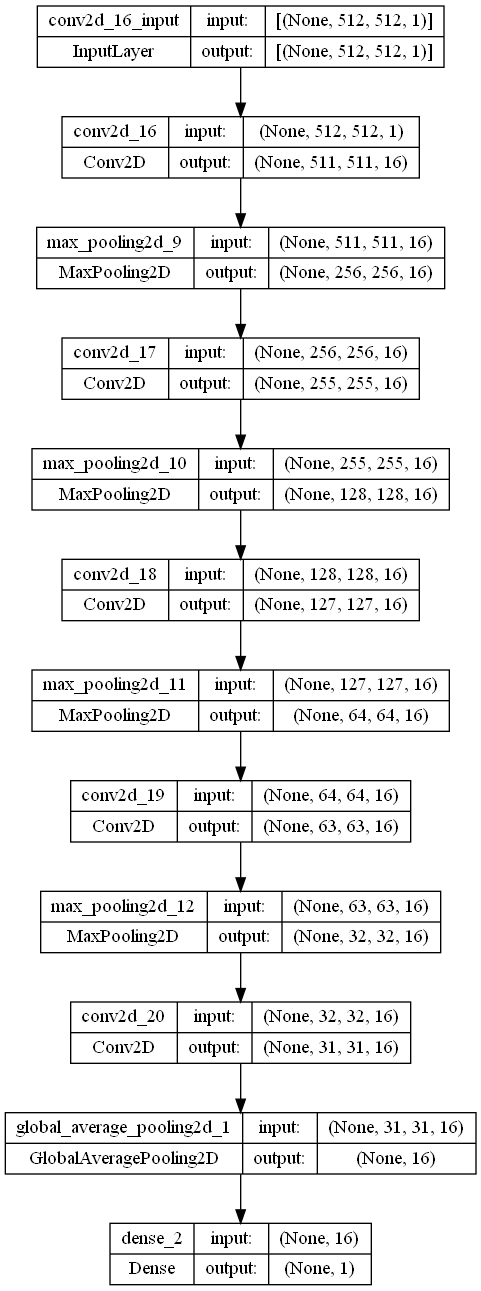
\includegraphics[width = 0.5 \textwidth]{walle_net_different.png}%walle_net.png
	\caption{Network Structure Bone}
	\label{fig:walle_net}
\end{figure}%

\begin{comment}
\section{receptive field}
%receptive field 
In recent years the depth of network increased drastically. In fact, \cite{Richter2021} stated that networks can be too deep. The features a convolution layer can process are limited by a parameter which is called receptive field. It predicts which layers won't contribute qualitatively to the accuracy.

\begin{align}
	r_l = r_{l-1}+((k_l-1)\prod_{i=0}^{l-1}g_i)
\end{align}

The values needed to calculate the function are the receptive field size of the previous layer r$_{l-1}$ which is 1 for r$_0$, g$_i$ the stride of layer i and k$_l$ the kernel size of layer l.

When the input resolution i is smaller than the previous receptive field size the so called border layer is reached.

\begin{align}
	r_{l-1} > i
\end{align} 

This layer separates the so called unproductive layers from the productive layers. \cite{Richter2021} states that with this layer it is possible to determine that every following layer will not contribute qualitatively to the test accuracy.
\end{comment}


%TODO: \cite{Szegedy_2015_CVPR} GoogleNet

\chapter{Methods and experimental Setup }
%TODO: this is not fitting anymore
To develop the network and compare it, multiple steps are necessary. First of all, several measures are chosen to compare the networks structures with each other. Afterwards, different augmentation techniques are tested. To compare the performances we will look at the test and training set performance side by side. The side by side comparison can give valuable information on how the network learns, especially when identifying overfitting. Next the learning performance of the network needs to be evaluated. This includes the use of fixed and decaying learning rates. After these fundamental evaluations starts the testing of the effect different changes in the network structure have on its performance. The extracted information of those tests is then used to develop and test a final batch of networks.

\section{Performance Measures}
%In order to facilitate a meaningful comparison between our networks and the one presented in \citet{Walle2023}, it is essential to evaluate mutual metrics.

To assess the performance of the networks, it is necessary to evaluate the discrepancy between the networks' outputs and the expected outputs. One common approach is to calculate the accuracy of the predictions made by the network, which is determined by the proportion of correctly classified samples to the total sample space.

\begin{align}
	Accuracy = \frac{correct\text{ } classifications}{all\text{ } classifications}
\end{align}

The accuracy measure can be misleading, particularly in the context of medical imaging, due to the sometimes extreme uneven distribution of data. In the event that a dataset is imbalanced, a network may achieve a high degree of accuracy by classifying each input as the most common occurring output.

%F1-score and Cohen's kappa are calculated to get a better understanding on how the actual performance of the network looks like. Accuracy is a commonly used metric which can give a general understanding of the overall performance.



%Considering that the targeted issue is in medical imaging, accuracy is not sufficient, it doesn't inform about the distribution of true positives and true negatives. In the medical research field the Cohen's kappa coefficient is applied which is developed to measure the agreement between two or more raters. It's uniqueness is given by taking the agreement by chance into account. Still it can sometimes be difficult to interpret. 
%Therefore, the F1-score is implemented as a third metric. This measure can be applied in situations where there is an imbalance between classes, which is true in the present case. It is calculated from the precision and the recall of the test set and can  be applied as a convenient metric for comparing and communicating the overall performance of a classifier. 


%\section{Performance Measures}
% performance measures for models and how to sufficiently compare networks
%When training networks a crucial step is to compare different network structures and their performances with each other to get the best results. One possibility is to introduce a measure that is capable to express how well a network would perform on new, unseen data. The most common way, which is employed in the majority of machine learning papers, is to calculate the accuracy of a network. This is done by splitting the data into two sets of arbitrary sizes. The first set inherits 80 percent of the data and is harnessed to train the network. The second set is then used to calculate the accuracy this is done by taking the proportion of correctly classified samples to the whole sample space. This measure can be misleading especially in medical imaging due to the sometimes extreme uneven distribution of data. 

%As an example if we have 1000 labeled images with 990 positive and 10 negative labeled images we could simply get a 99 percent accuracy by only outputting positives. This accuracy is in general true but if for example the network is suposed to detect if a tumor is seen in the image and we have 10 examples where a tumor should be detected, it would be way more important to detect the tumors and get a lower accuracy then not detecting the tumors at all. Since our data is also quite imbalanced a different measure needs to be used to compare networks with each other.
%TODO: not sure if the example is correct since im not sure if the f1 score measure helps with the issiue 

\subsection{Cohen's Kappa}
%TODO: needs to be finished 
%A different measure which was initially introduced as a measure of agreement between observers of psychological behavior, is the degree of agreement between two or more people observing the same experiment. This measure is called Cohen's kappa. It's application in machine learning is quite easy to implement since there are at least two observers given by the labeled data and the results of the machine learning model.
%Considering that the targeted issue is in medical imaging, accuracy is not sufficient.
In the field of medical research, the Cohen's kappa coefficient is employed to assess the degree of agreement between two or more raters. Its distinctive feature is the incorporation of an element of chance into the calculation of the agreement. However, it should be noted that the interpretation of the results can sometimes prove challenging. 

\newcommand{\STAB}[1]{\begin{tabular}{@{}c@{}}#1\end{tabular}}
\begin{center}
	\begin{tabular}{ccccccc}
		\hline
		&&&&\multicolumn{3}{c}{\textbf{Observer 1}}\\
		&&&&false&true&Total\\
		\hline
		\textbf{Oberver 2}&&false& &A &B &A+B \\
		
		&&true&&C&D&C+D\\
		
		&&Total&&A+C&B+D&A+B+C+D\\
	\end{tabular}
\end{center}

The initial paper by \citet{Cohen1960} introducing this measure suggests that for any problem in nominal scale agreement between two entities, there are only two relevant quantities. The first of these is the total agreement, $p_0$, which is equivalent to the previously defined accuracy. The second measure, $p_c$, is the proportion of units for which the agreement is expected by chance. This is also supported by \citet{Vieira2010}, which states that it is thought to be a more robust measure than a simple percent agreement calculation.

\begin{align}
	p_c =\frac{(a+b)\cdot(a+c)+(c+d)\cdot(b+d)}{(a+b+c+d)^2}
\end{align}

Consequently, the proportion of agreement, $\kappa$, represents the degree of consensus that remains after the influence of chance has been excluded. 
%Cohen's Kappa 

\begin{align}
	\kappa = \frac{p_0-p_c}{1-p_c}
\end{align}

\subsection{F1-Score}
Another metric that may be employed is the F1-score. This metric can be employed in scenarios where there is an unequal distribution of instances across classes. The F1-score is calculated from the precision and recall of the model and can be applied as a convenient metric for comparing and communicating the overall performance of a classifier. 

\begin{center}
	\begin{tabular}{c||c|c}
		
		& &\\
		Total Population	& Predicted Positives & Predicted Negatives  	\\
		= N+P & (PP) &(PN)\\
		\hline
		\hline
		& &\\
		Positives &  True Positives& False Negatives   \\
		(P)& (TP)&(FN)\\
		\hline
		& &\\
		Negatives & False Positives  & True Negatives  	\\
		(N)&(FP) &(TN)\\
	\end{tabular}
\end{center}

%F1Score



%A categorical measure which is especially used in imbalanced classes is the F1 score.It is often implemented, since the measure can also be applied in a multi class environment. This measure is the harmonic mean of precision and recall: %TODO: go more into detail with the muklticlass environment 

Precision is defined as the ratio of true positives to the total number of positives predicted.
\begin{align}
	Precision = \frac{TP}{TP+FP}
\end{align}

The recall ratio represents the proportion of true positives among all the positives in the ground truth.

\begin{align}
	Recall = \frac{TP}{FP+FN}
\end{align}

\begin{align}
	F1\text{-}Score = 2\cdot \frac{precission\cdot recall}{precission+recall}
\end{align}

Consequently, multiplication is employed in the numerator, whereby the measure is likely to approach zero if one of the measures is close to zero. Consequently, it is crucial to achieve a balance between the two scores in order to obtain a higher total. This implies that the issue pertaining to the utilisation of accuracy is negated, as a balanced detection is essential for attaining a higher score. Nevertheless, categorical measures, such as the F1-score, do not provide a comprehensive understanding of a network's performance.

In the case of each data point, it is simply classified as either correct or incorrect, without consideration of the magnitude of the error. This is because each data point is either correctly or incorrectly classified, without consideration of the magnitude of the error \citep{Dinga2019}. 


\section{Existing Network Structure}
The initial approach of \citet{Walle2023} set the output size to five since the scans had five severity grades. This approach only yielded a low accuracy. Considering that the most significant information is if a re-scan is necessary or not the output size was changed to one, which yielded significantly better results. Accordingly, in this thesis an output size of one is implemented for the scans.

\section{Loss}
As a loss function the weighted binary cross entropy loss is chosen. Since the input data is not equally distributed this is meant to help the network shift into a more generalized direction.

\section{Data}
\begin{center}
	\begin{tabular}{||c|c|c||c||}
		
		Motion Grade&  Tibia rounded& Radius rounded & Sum 	\\
		\hline
		\hline
		1 &  243&  45& 288   \\
		\hline
		2 &  171 & 102&  273\\
		\hline
		3 &  57&  173&  230 \\
		\hline
		4 &   25 & 148&  173 \\
		\hline
		5 &  4& 32&   36\\
		\hline
		\hline
		Sum&500&500&1000\\
		
		\hline
	\end{tabular}
\end{center}

The data utilized is provided by the osteology department of the Unfallklinikum Hamburg-Eppendorf and labeled by 3 different professionals.
The labeled data contains 500 scans of the radius and 500 scans of the tibia. In  40.2\% of all scans the doctors had an agreement, 41.4\% for grading the tibia and 39\% for grading the radius. 

Considering the case that one doctor was for or against a re-scan contrary to the other 2 doctors it is observed, that this happens in 26 cases for the tibia and 109 cases for the radius. This makes it hard to compare in view of the significantly bigger amount of values in the domain of 3 and 4 for the radius compared to the tibia. By linking the amount of values where the rounded gathered rating was 3 or 4 to the possibility of a re-scan we get 31.7\% for tibia and 33.9\% for the radius.  %TODO this text need to be rewritten because of lack of motivation

For training the network the radius scans are selected as those are more equal distributed. Tibia is not considered because the use of both sets together lead to a worse accuracy.

The data is separated in a test and training set. The training set consists of 75\% of the data and test set of the remaining 25\%. The training data was then augmented. The test data is not augmented because in a real world example the augmented scans are unlikely to appear and would thereby perturbed the results.

\section{Early Stopping and Overfitting}
% early stopping / overfitting 
When training a network with insufficient data, the method of early stopping is typically employed. This technique is utilized in machine learning to prevent overfitting during model training. Overfitting occurs in machine learning when a model learns to perform well on the training data, capturing noise and irrelevant patterns, but performs poorly on new, unseen data. This indicates that the model has memorized the training data instead of learning the underlying patterns, leading to reduced generalization ability and diminished predictive accuracy on real-world examples. The technique of early stopping involves monitoring the performance of a model on a validation data set and halting training when the performance on the validation data set begins to deteriorate. By preventing excessive training, early stopping enables a model to generalise more effectively to new data and to improve its ability to make accurate predictions on new data. This technique strikes a balance between training optimal performance and avoiding the point where the model begins to memorise noise in the training data.


\section{Batch Normalization}
%Batch Normalization
To ease the training process the initial values of the networks parameters are typically normalized by initializing them with zero mean. By training on our data we would usually lose this normalization, which slows down training and amplifies changes as the network becomes deeper. To remove those effects and therefore enhance the training stability and convergence of deep neural networks, batch normalization can be employed. \citet{Ioffe2015} By standardizing the inputs within each mini-batch during training, gradient related issues are mitigated and convergence is  accelerated. Additionally, it acts as a form of regularization and curbs overfitting. With this method we are able to use higher learning rates and pay less attention to the initialization parameters. \citet{Ruder2016} 

\section{Weight Initialization}
The weight initialization which is employed for all networks is the preset weight initialization technique used in the Flux.jl library. It  is described in \citet{glorot2010}. This method draws random numbers from a uniform distribution on the interval [-x,x] where:

\begin{align}
	x = gain \cdot \sqrt{\frac{6}{fan\_in + fan\_out}}
\end{align}  

The gain factor is preset to one, fan$\_$in is the number of input neurons connected to one output neuron and fan$\_$out is the number of output neurons connected to one input neuron.


\section{Transfer Learning}
%Transfere Learning 
Due to the lack of training data a possible method of enhancing the network is using transfer learning. This method is a common and effective strategy to use before training a network on a small data set. By pre-training the network on extremely large datasets like ImageNet with 1.4 million images and 1000 classes, trying to learn generic features that can be shared among networks \citep{Yamashita2018}. This is a unique advantage of deep learning that makes itself useful in various domain tasks with small datasets. Despite the popularity of transfer learning in medical imaging there hasn't been a lot of work studying of its effects. Usually transfer learning is performed by taking a standard IMAGENET architecture with pre-trained weights and then fine tuning its parameters on the data set which the network is supposed to detect.
%When comparing medical datasets with IMAGENET we can see that medical images usually range from a few hundred to a couple hundred thousands  (not sure if i want to go in this direction)


\citet{Raghu2019} shows on two large scale medical image networks that the gain of transfer learning on those networks is marginal. It also shows that transfer usually helps large scale models, with small models showing little difference. Therefore, transfer learning is not applied in this study.

\section{Hardware}
For our training we used a "Nvidia Geforce RTX 2070 Super". It has 8 gigabytes of graphic memory. We decided to use a batch size of 16 images per iteration and a training set of 3200 images per Epoch. 

\section{Data Augmentation}
Considering that the data set only consists of 500 radius scans the data set was enlarge by different augmentation methods. Meanwhile not every method is suitable for any type of data. Different augmentation methods are compared and will be evaluated in the results. The outcome shows that the optimal set of augmentation methods consists of:

\begin{itemize}
	\item 90$^{\circ}$ rotation
		\item the use of cropped image snippets 
	\item flipping of the image
	\item Gaussian noise

\end{itemize}

The implementation for Gaussian noise, 90$^{\circ}$ rotation and flipping of the images can be found in Julia libraries. The cropping of the image snippets is not as trivial. First, a minimal image size of 620 pixels is defined being the smallest frame where all the information is kept. The maximal size is limited by the input image size of 1536x1536 pixels. The decision on the frame size is made by a random normal distribution. Depending on the resulting size, the frame is randomly moved in horizontal or vertical direction, whilst always retaining the necessary information.
%TODO: generate image that shows how the important information can be retained 

\section{Data Augmentation}
%imbalanced data in medical imaging   
Commonly, biological data tends to be imbalanced. Often negative samples are more common, than positive ones \citep{Alzubaidi2021}. When training a network with imbalanced data, the network is prone to bias towards the major classes, since it prioritizes learning the features for detecting those classes. This also means that the network does not get enough exposure to detect minor features and therefore can't learn its distinctive features. All this leads to a higher number of false negatives. With the network trying to capture the minor features it can run into the issue of overfitting the network. In our case there is a lack of data that is labeled with the severity type of 1 and 5. This holds a major issue, since type 5 scans are in need of a re-scan. Thus, a high accuracy score for detecting this class to be sure that healthcare professionals won't unnecessarily re-scan patients is desirable. A high accuracy score in class detection could thereby reduce the patient's exposure to unnecessary radiation.%TODO: ausschmücken informationsdichte ist zu hoch 


%Data Augmentation
In medical imaging the issue of imbalanced data is often combined with the lack of training data. When training a CNN with to little data we have to stop early and don't get an optimal accuracy for the network. Further training would lead the network to overfit and lose its validity. A common solution for this issue is the augmentation of the training data. Most augmentation techniques are based on basic image manipulations and generic translations. In this paper some of the techniques contained in \citet{Shorten2019} will be used.\citet{Shorten2019} state that the most common method to augment data is the horizontal and vertical flipping of the images, where horizontal flipping is the most common implementation.

Another method is to crop the central patch of the image. This can be implemented as random cropping where a batch of variable size is cut from the main image and then scaled to the input size. This provides a quite similar effect as translation. 

Translation shifts the image left, right, up and down. Because the data in our set is centered the positional bias of the network can be reduced by applying this method. Usually the remaining space would be filled up with zeros or random Gaussian noise. Since the given dataset contains large images with the important information lying in the center a mix of cropping and translation is applied to stay in the bounds of the image so that adding padding to the image isn't required. 

Rotation can also be implemented as an augmentation technique. The rotation can be chosen between 1 and 359$^\circ$. This method needs to be handled with care. A common example are the numbers from the MNIST data set which would change their label when rotated to a certain degree. This method is also adapted by \citet{Zhang2020}, examining cardiac magnetic resonance T1 mappings, which only adds a $\pm$ 5 $^\circ$ uniform distributed rotation as their data augmentation methods. 



\subsection{Optimizer}
Commonly, Adam is used with a fixed learning rate of 0.001 which is sufficient in most cases. In the initial tests conducted with a learning rate of 0.001, the standard derivation of loss and accuracy is significant leading to the investigation on the learning rate. A strong oscillating loss or accuracy is usually the case when a network is trained with a learning rate that is too high. The learning rate determines how fast or slow the network will converge towards the optimal weights. A learning rate which is too large might lead the network to overshoot. This can either result in oscillation or in some extreme cases to a diverging network. In consequence different learning rates and methods are tested. The conducted tests used Adam and ADAMW with the possible addition of different weight decay parameters. Either a fixed value or a starting parameter which then applied an epoch wise decay function is chosen. These tests are conducted on the network of \citet{Walle2023} and trained for 60 epochs to get a general understanding of the parameters performances.


\section{Network Building Blocks}
Subsequently, the different building blocks or methods to be included in the network are tested as follows:

\begin{itemize}
	\item Inception Block 
	\item increasing the network depth
	\item addition of Skip Connections
	\item variation in the number of filters
\end{itemize}

Building a network from scratch can be a difficult task, hence the network from \citet{Walle2023} was implemented as a start point. Due to the many possible combinations that could be changed, only small changes to the network are made before training it for 60 epochs. This way a general understanding on the performance of certain components could be obtained without needing to wait a long time for the training to complete. 

The information gathered in this approach are used to build a set of final networks which are trained for 200 epochs and then compared with the findings of \citet{Walle2023}.


%TODO: check if i want to include weightinitialization in my setup
%Before a network can be trained the weights of the neurons have to be initialized, in general there are three possible methodes that can be used. The first method initializes all the weights of the network with zeros, this has the issue that the back propagation would calculate the same update parameter for each of the layers. The resulting symmetry wouldn't break through out the training process\cite{Narkhede2021}.










\chapter{Results}

%I used the network structure given by \cite{Walle2023} as a reference network and trained it for 200 epochs with different augmentation compositions. Since the results of the paper showed that the network structure could perform well on the given image data I was able to use it to establish a augmented dataset that was optimized for training. This data set could then be used to train different type of networks. By looking at the change and maximum values of the kohen's kappa and accuracy and minimum for loss of the test set. With those information, I was able to extract which methods worked well for training which ensure a stable growth  and also result in higher maximum accuracy and kohen's kappa. Since the used Scans had a depth of 110 layers we were able to extract multiple images from one scan. To stay comparable with \cite{Walle2023} I also used 8 equally separated slices from every image, since I also saw the danger of taking to many images of one scan which might mean that the images could be to similar for the network and have no benefits when training. 
%The data  Augmentation methodes i trialed where :
\section{Augmentation Tests}
The first milestone of this thesis was to replicate the results of \citet{Walle2023}. The networks displayed in \ref{fig:walle_net}, which will later be refered to as the initial model, was chosen with the output size as one. Consequently, the softmax function is not applied as the last layer activation function but sigmoid. This output size is chosen because it is more valuable to detect if a re-scan is necessary than the exact severity level. Furthermore, the results of \citet{Walle2023} show that the accuracy of the model significantly increases with the reduction of the output size.

In our first test different combinations of augmentation techniques are employed in combination and trained on the model of \citet{Walle2023} for 200 epochs. Aiming to find the best augmentation method for the data. In general, the following augmentation techniques are applied to the training data: 


\begin{itemize}
	\item rotation by 90$^{\circ}$,180$^{\circ}$ and 270$^{\circ}$
	\item rotation by 1-359$^{\circ}$
	\item flipping image horizontal or vertical 
	\item taking image snippets and resizing them 
	\item addition of Gaussian noise 
\end{itemize}

\begin{figure}
	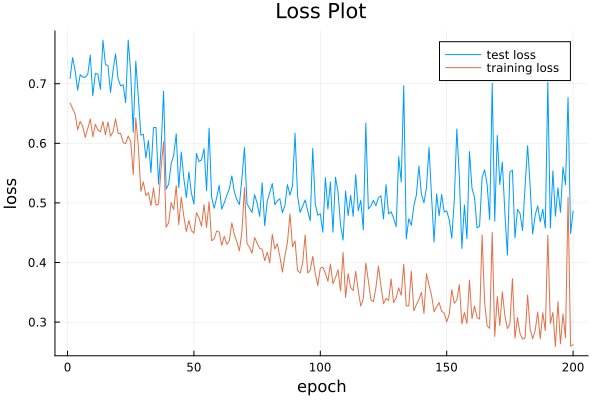
\includegraphics[width=0.4\linewidth]{loss_png_final_run_0_7.png}\hfill
	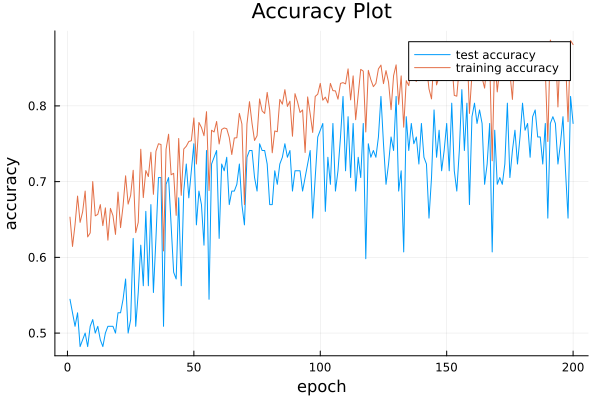
\includegraphics[width=0.4\linewidth]{accuracy_png_final_run_0_7.png}
	\\[\smallskipamount]
	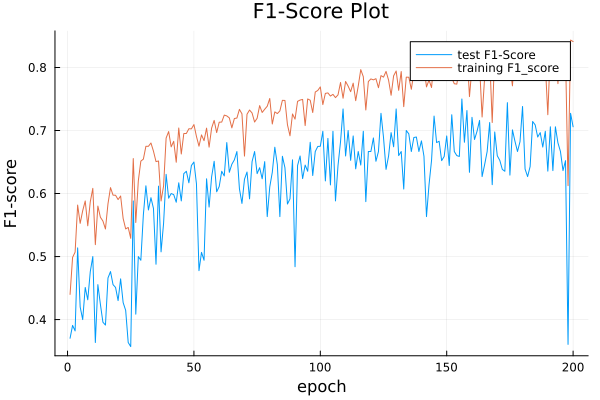
\includegraphics[width=0.4\linewidth]{f1_score_png_final_run_0_7.png}\hfill
	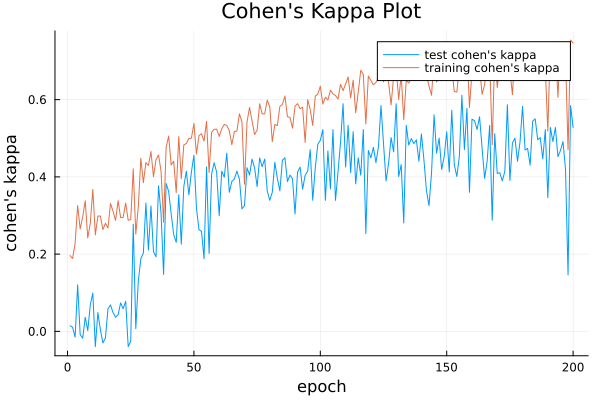
\includegraphics[width=0.4\linewidth]{cohens_kappa_png_final_run_0_7.png}
	\caption{90$^{\circ}$ rotation, flipping and Gaussian noise (epochs: 200 loss: $53.1\pm8.12\% $ accuracy: $74.9\pm5.8\%$ F1-score: $62.5\pm13.4\%$  Cohen's kappa: $44\pm15.4$ )}
\end{figure}%

\begin{figure}
	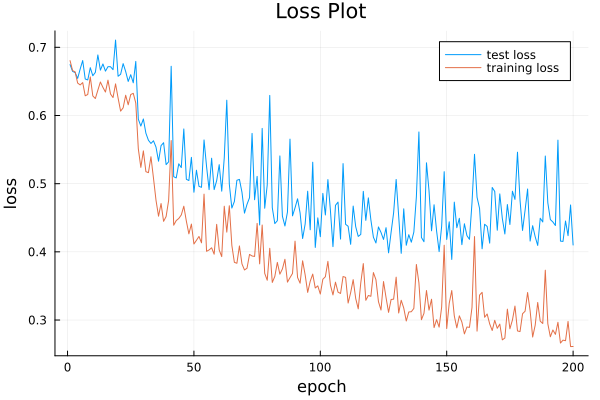
\includegraphics[width=0.4\linewidth]{loss_png_final_run_6_2.png}\hfill
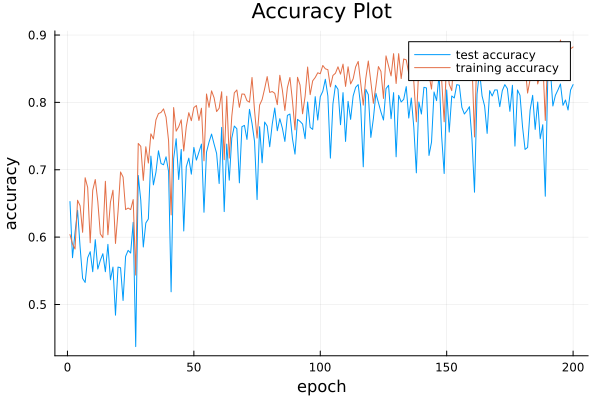
\includegraphics[width=0.4\linewidth]{accuracy_png_final_run_6_2.png}
\\[\smallskipamount]
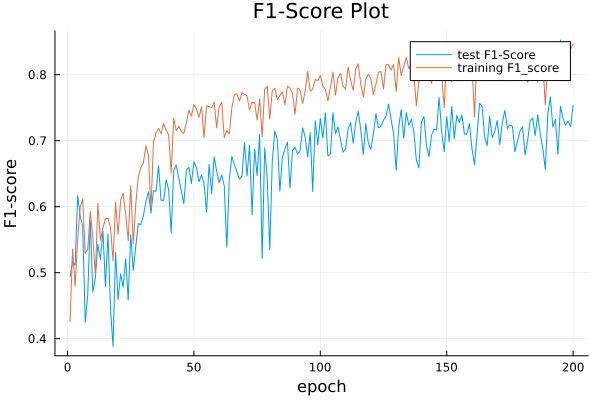
\includegraphics[width=0.4\linewidth]{f1_score_png_final_run_6_2.png}\hfill
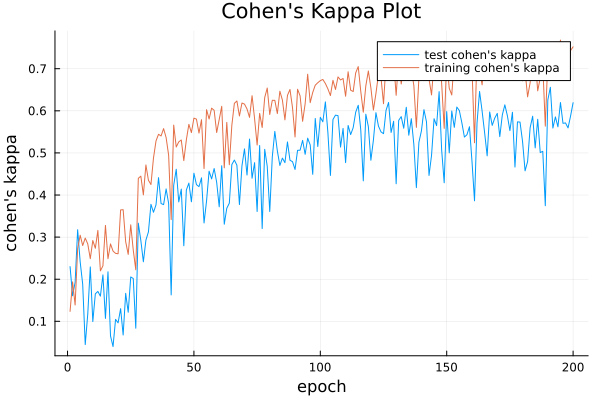
\includegraphics[width=0.4\linewidth]{cohens_kappa_png_final_run_6_2.png}
	\caption{90$^{\circ}$ rotation, resized image snippets, flipping and Gaussian noise(epochs: 200 loss: $43\pm2.3\% $ accuracy: $81\pm1.6\%$ F1-score: $73.6\pm1.4\%$  Cohen's kappa: $58.8\pm2.6$ )}
\end{figure}%

\begin{figure}
	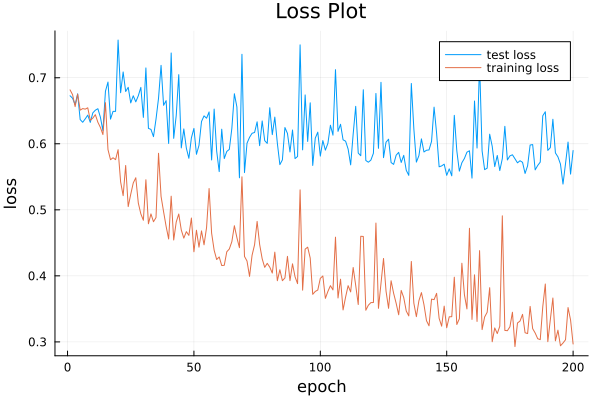
\includegraphics[width=0.4\linewidth]{loss_png_final_run_0_5.png}\hfill
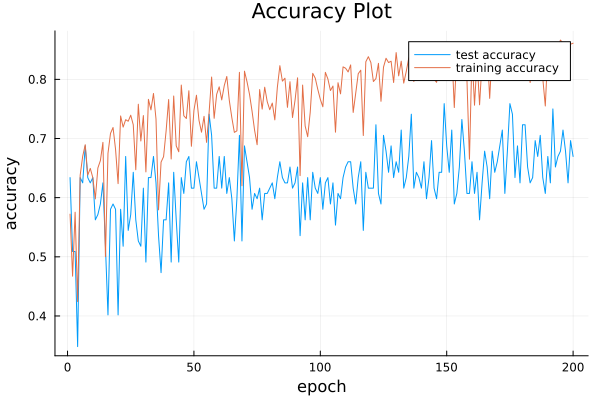
\includegraphics[width=0.4\linewidth]{accuracy_png_final_run_0_5.png}
\\[\smallskipamount]
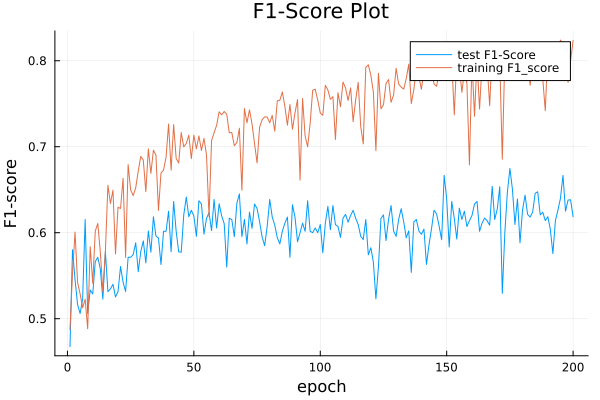
\includegraphics[width=0.4\linewidth]{f1_score_png_final_run_0_5.png}\hfill
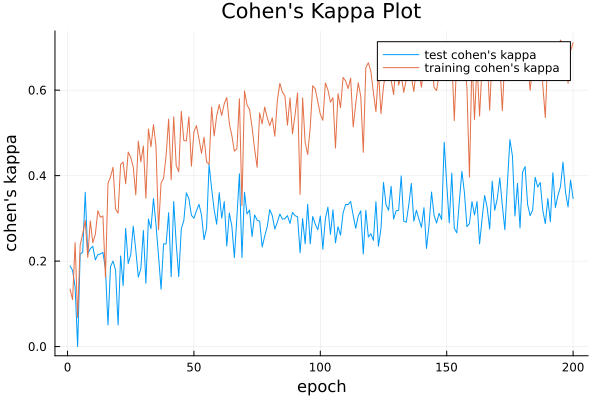
\includegraphics[width=0.4\linewidth]{cohens_kappa_png_final_run_0_5.png}
	\caption{1-360$^{\circ}$ rotation, resized image snippets,flipping and Gaussian noise(epochs: 200 loss: $57.1\pm2.3\% $ accuracy: $67.7\pm3\%$ F1-score: $63.8\pm1.7\%$  Cohen's kappa: $37.1\pm3.7$ )}
\end{figure}%

\begin{figure}
	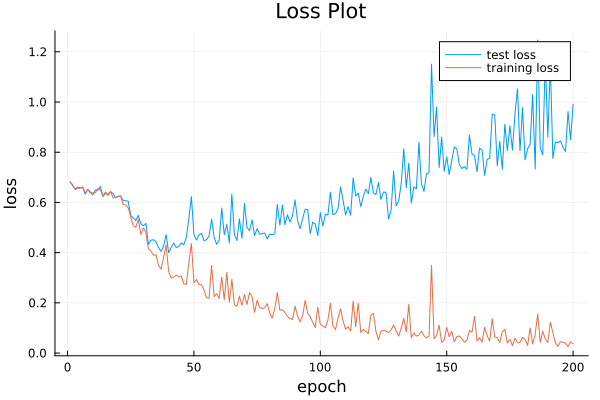
\includegraphics[width=0.4\linewidth]{loss_png_final_run_0_4.png}\hfill
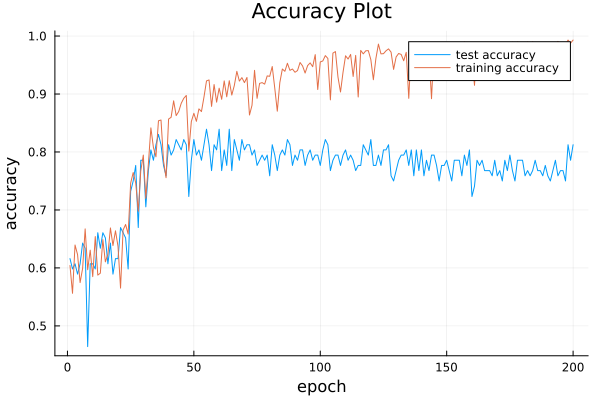
\includegraphics[width=0.4\linewidth]{accuracy_png_final_run_0_4.png}
\\[\smallskipamount]
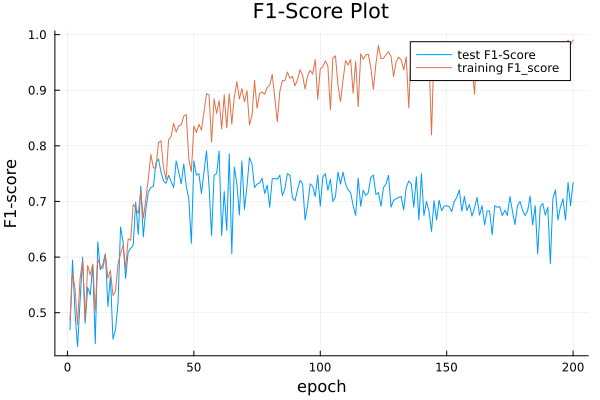
\includegraphics[width=0.4\linewidth]{f1_score_png_final_run_0_4.png}\hfill
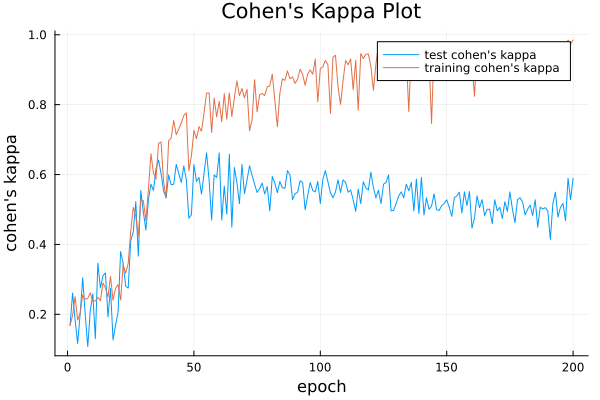
\includegraphics[width=0.4\linewidth]{cohens_kappa_png_final_run_0_4.png}
	\caption{$\pm$5$^{\circ}$ rotation, resized image snippets, flipping and Gaussian noise(epochs: 200 loss: $87.9\pm7.8\% $ accuracy: $78.3\pm2.6\%$ F1-score: $70.4\pm2.7\%$  Cohen's kappa: $53.3\pm4.8$ )}
\end{figure}%

\begin{figure}
	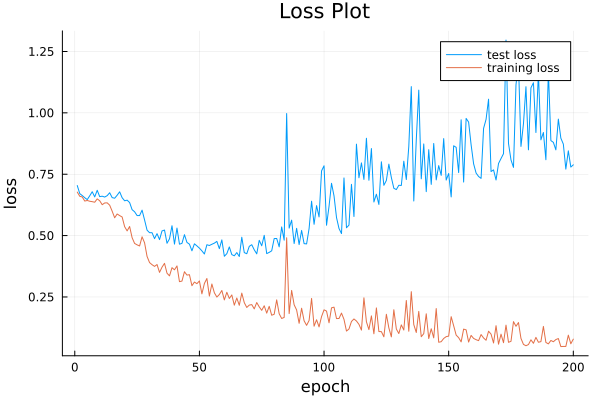
\includegraphics[width=0.4\linewidth]{loss_png_final_run_0_6.png}\hfill
	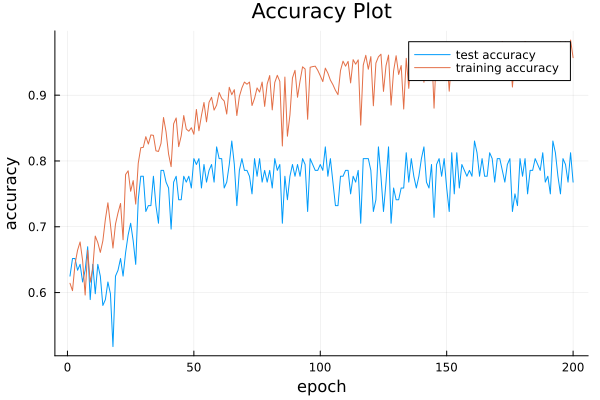
\includegraphics[width=0.4\linewidth]{accuracy_png_final_run_0_6.png}
	\\[\smallskipamount]
	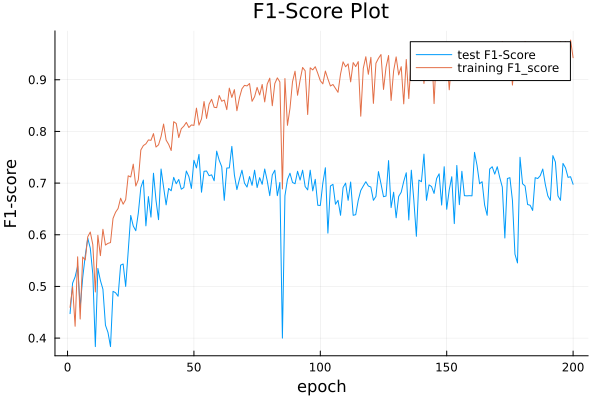
\includegraphics[width=0.4\linewidth]{f1_score_png_final_run_0_6.png}\hfill
	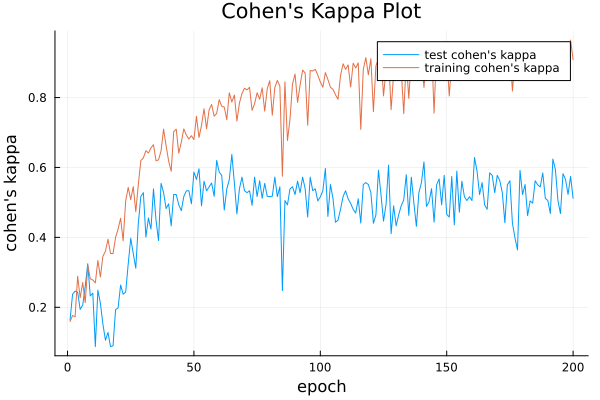
\includegraphics[width=0.4\linewidth]{cohens_kappa_png_final_run_0_6.png}
	\caption{resized image snippets, flipping and Gaussian noise(epochs: 200 loss: $82.5\pm5.3\% $ accuracy: $78.3\pm2.4\%$ F1-score: $71\pm2.5\%$  Cohen's kappa: $53.8\pm44.3$ )}
\end{figure}%

	\clearpage

%TODO: this part needs to be rewritten 
The simultaneous use of rotation by 90$^{\circ}$, 180$^{\circ}$ and 270$^{\circ}$, flipping the image horizontal or vertical, adding Gaussian noise, taking image snippets and resizing them results in a stable training with the greatest accuracy and Cohen's kappa values. It is observed that the addition of 1-360$^{\circ}$ rotation is seemingly inefficient in training networks. When only using the $\pm$5$^{\circ}$ rotation described in \citet{Zhang2020}, the network reaches similar peak values in training but quickly starts to diverge after less than 50 epochs. It still shows little oscillation.

\begin{figure}[h]
	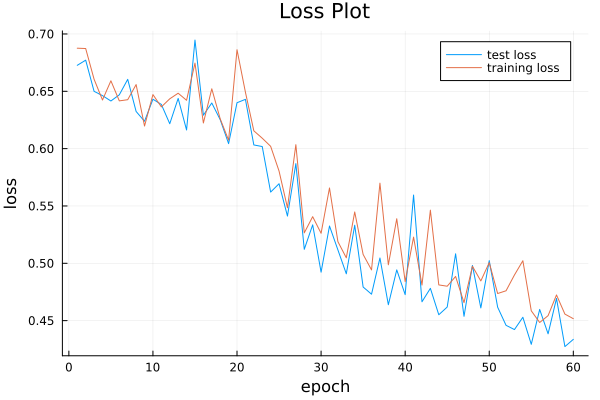
\includegraphics[width=0.4\linewidth]{loss_png_11_1.png}\hfill
	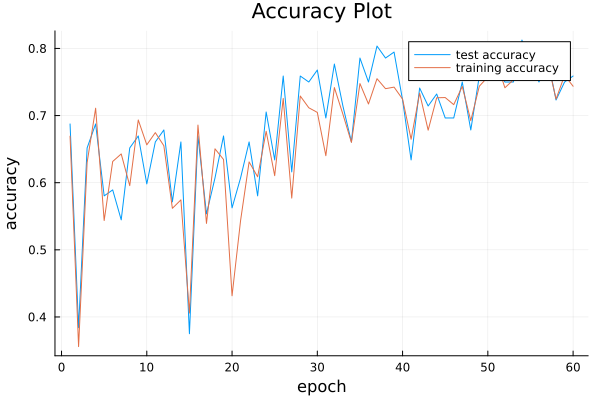
\includegraphics[width=0.4\linewidth]{accuracy_png_11_1.png}
	\\[\smallskipamount]
	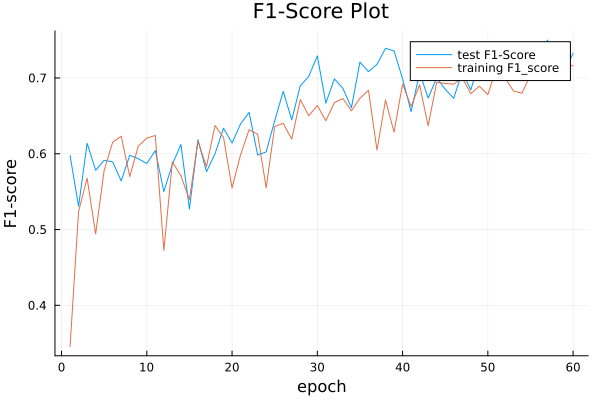
\includegraphics[width=0.4\linewidth]{f1_score_png_11_1.png}\hfill
	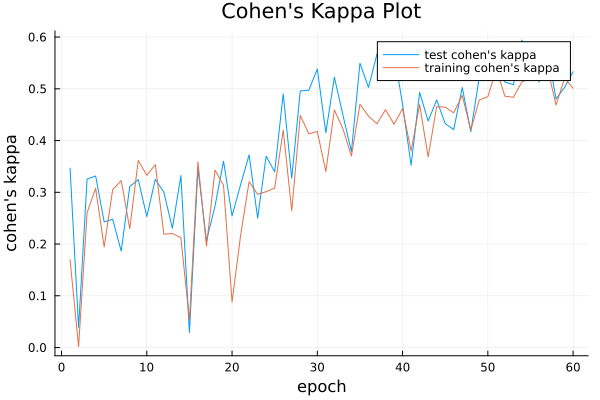
\includegraphics[width=0.4\linewidth]{cohens_kappa_png_11_1.png}
	\caption{Adam without learning rate reduction(epochs: 60 loss: $44.3\pm1.7\% $ accuracy: $75.7\pm2.2\%$ F1-score: $72.6\pm1.6\%$  Cohen's kappa: $52.6\pm3.4$ )}
\end{figure}%

\begin{figure}[h]
	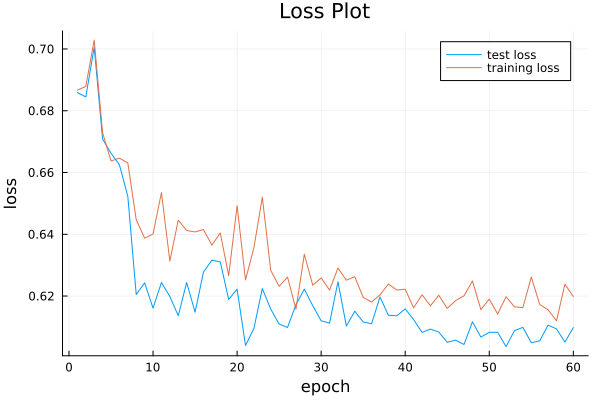
\includegraphics[width=0.4\linewidth]{loss_png_11_2.png}\hfill
	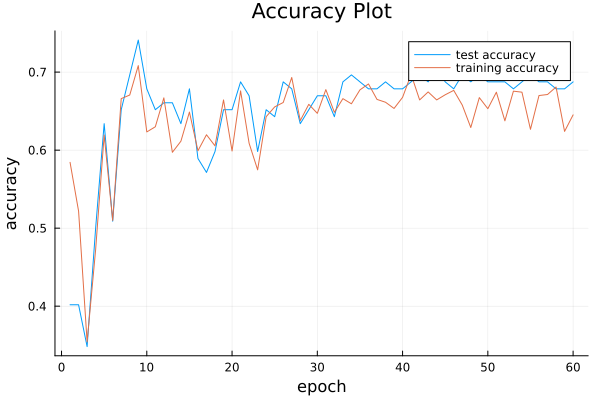
\includegraphics[width=0.4\linewidth]{accuracy_png_11_2.png}
	\\[\smallskipamount]
	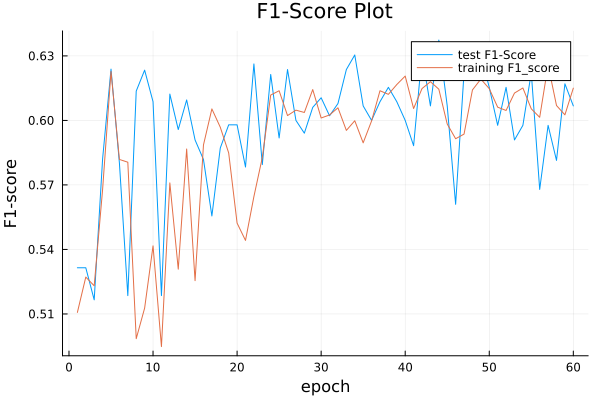
\includegraphics[width=0.4\linewidth]{f1_score_png_11_2.png}\hfill
	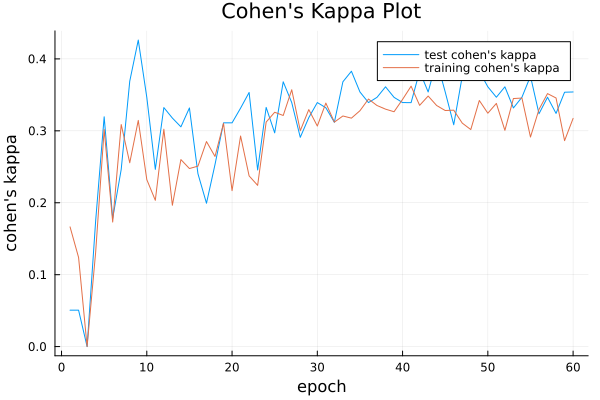
\includegraphics[width=0.4\linewidth]{cohens_kappa_png_11_2.png}
	\caption{Adam with learning rate reduction of 0.94 per Epoch(epochs: 60 loss: $60.8\pm 0.3\% $ accuracy: $68.6\pm6.7\%$ F1-score: $59.9\pm2.1\%$  Cohen's kappa: $34.6\pm2$ )}
\end{figure}%

\begin{figure}[h]
	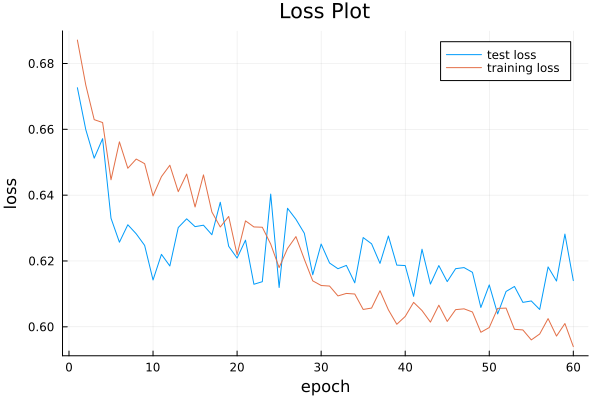
\includegraphics[width=0.4\linewidth]{loss_png_11_3.png}\hfill
	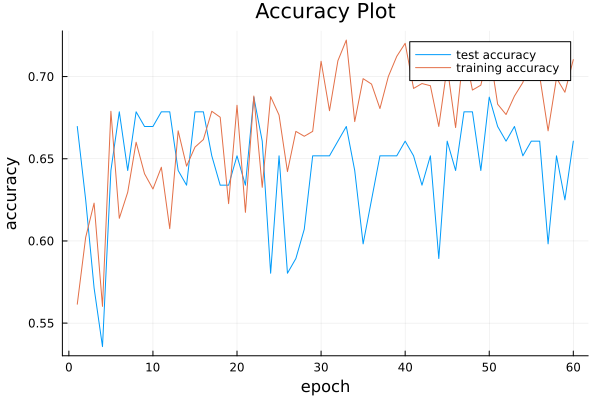
\includegraphics[width=0.4\linewidth]{accuracy_png_11_3.png}
	\\[\smallskipamount]
	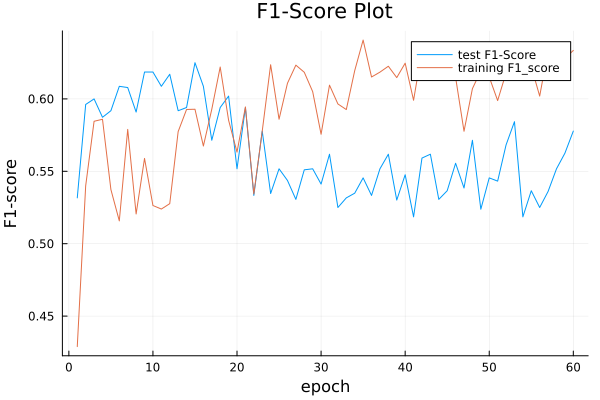
\includegraphics[width=0.4\linewidth]{f1_score_png_11_3.png}\hfill
	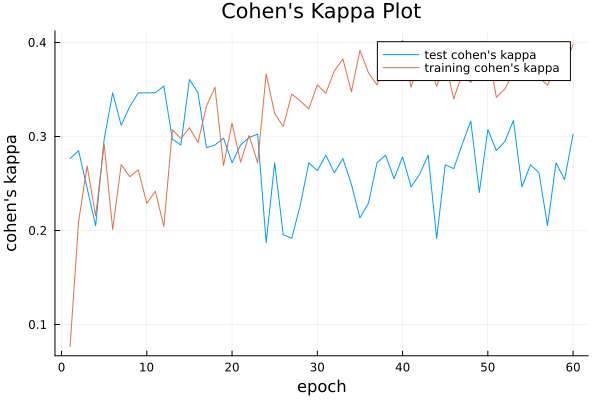
\includegraphics[width=0.4\linewidth]{cohens_kappa_png_11_3.png}
	\caption{ADAMW with learning rate reduction of 0.94 per epoch(epochs: 60 loss: $61.5\pm0.8\% $ accuracy: $64.3\pm2.6\%$ F1-score: $54.8\pm2\%$  Cohen's kappa: $26.1\pm3.2$ )}
\end{figure}%

\clearpage
\section{Optimizer Tests}
Due to the oscillation of the model the effect of adapting the learning rate over time is tested. When comparing the different learning models with each other it is clear that Adam, with a fixed learning rate, outperforms the two competing methods. After 60 epochs of training it has the lowest loss and the highest accuracy. It also seems to converge since the loss is decreasing in a somewhat linear manner. The other measures are also steadily increasing. This is different for Adam where a learning rate reduction of 0.94 per epoch is used equaling a learning rate decrease of 0.1 every 35 epochs. This method appears to quickly converge in the first 10 epochs and afterwards it slows down significant. If we look at the learning rate a major decrease in the first 10 epochs from 0.7 to 0.62 is observed. In the following 50 epochs it merely decreases by 0.02. This stagnation is also seen in the accuracy F1-score and Cohen's kappa without gaining a lot after the 10th epoch. A possible reason is that Adam's learning rate is not decoupled from the gradient based update method. Therefore, the performance of ADAMW with a learning rate decrease of 0.94 per epoch is analyzed. When looking at the loss of the network a somewhat steady decrease is detected which is not as fast as regular Adam. Although the learning rate is lower, the loss might decrease slower as well. By analyzing the other measures, it is apparent that after epoch 20 the results of the test set compared to the training set get worse. Thereby the results for the test set are decreasing while the ones for the training set increase slowly, with strong oscillation. Consequently, in the next tests Adam will be applied without a learning rate decrease. Still sometimes a learning rate of 0.0001 is implemented instead of the standard learning rate of 0.001. Due to the fact that bigger networks need a smaller learning rate because the network won't converge otherwise.



After the decision on the optimizer, it is tested which network structures performs well on the training data. In view of the many different setups to test, it is determined to train every network for 60 epochs. First of all, small changes are implemented into the network. Thereby the impact of adding and changing different layers on performance of the network can be detected. Here is a list of the building blocks:

\begin{itemize}
	\item inception block 
	\item shortcut connection
	\item additional convolution layers
	\item adding of padding 
	\item changing pooling layers by strided convolution 
	
\end{itemize} 
\begin{table}
\begin{tabular}{cccccc}
	\toprule
	\multicolumn{2}{c}{model 1} &\multicolumn{2}{c}{model 2} & \multicolumn{2}{c}{model 3} \\ 
	Layer & Output &Layer & Output &Layer & Output\\
	\cmidrule(l){1-2} \cmidrule(l){3-4}\cmidrule(l){5-6}
	Input&(,512,512,1)&Input&(,512,512,1)&Input&(,512,512,1)\\
	\cmidrule(l){1-2} \cmidrule(l){3-4}\cmidrule(l){5-6}
	Conv2D	& (,511,511,16) &Conv2D	& (,511,511,16)&Conv2D	& (,511,511,16)\\
	\cmidrule(l){1-2} \cmidrule(l){3-4}\cmidrule(l){5-6}
	MaxPool&(,256,256,16)&MaxPool&(,256,256,16)&MaxPool&(,256,256,16)\\
	\cmidrule(l){1-2} \cmidrule(l){3-4}\cmidrule(l){5-6}
	Conv2D&(,255,255,16)&Conv2D&(,255,255,16)&Conv2D&(,255,255,16)\\
	\cmidrule(l){1-2} \cmidrule(l){3-4}\cmidrule(l){5-6}
	MaxPool&(,128,128,16)&MaxPool&(,128,128,16)&MaxPool&(,128,128,16)\\
	\cmidrule(l){1-2} \cmidrule(l){3-4}\cmidrule(l){5-6}
	Conv2D&(,127,127,16)&Inception&(,128,128,16)&Conv2D&(,127,127,16)\\
	\cmidrule(l){1-2} \cmidrule(l){3-4}\cmidrule(l){5-6}
	MaxPool&(,64,64,16)&MaxPool&(,64,64,16)&MaxPool&(,64,64,16)\\
	\cmidrule(l){1-2} \cmidrule(l){3-4}\cmidrule(l){5-6}
	Conv2D&(,63,63,16)&Conv2D&(,63,63,16)&Conv2D&(,63,63,16)\\
	\cmidrule(l){1-2} \cmidrule(l){3-4}\cmidrule(l){5-6}
	MaxPool&(,32,32,16)&MaxPool&(,32,32,16)&MaxPool&(,32,32,16)\\
	\cmidrule(l){1-2} \cmidrule(l){3-4}\cmidrule(l){5-6}
	Conv2D&(,31,31,16)&Conv2D&(,31,31,16)&Conv2D&(,31,31,16)\\
	\cmidrule(l){1-2} \cmidrule(l){3-4}\cmidrule(l){5-6}
	Conv2D&(,30,30,16)&GAP&(,16)&Conv2D&(,30,30,16)\\
	\cmidrule(l){1-2} \cmidrule(l){3-4}\cmidrule(l){5-6}
	GAP&(,16)&Dense&(,1)&Conv2D&(,29,29,16)\\
	\cmidrule(l){1-2} \cmidrule(l){3-4}\cmidrule(l){5-6}
	Dense&(,1)&&&GAP&(,16)\\
	\cmidrule(l){5-6}
	& & & &Dense&(,1)\\
	%Todo GAP needs to be defined somewhere	 	
\end{tabular}

\begin{tabular}{cccccc}
	\toprule
	\multicolumn{2}{c}{model 4} &\multicolumn{2}{c}{model 5} & \multicolumn{2}{c}{model 6} \\ 
	Layer & Output &Layer & Output &Layer & Output\\
	\cmidrule(l){1-2} \cmidrule(l){3-4}\cmidrule(l){5-6}
	Input&(,512,512,1)&Input&(,512,512,1)&Input&(,512,512,1)\\
	\cmidrule(l){1-2} \cmidrule(l){3-4}\cmidrule(l){5-6}
	Conv2D& (,511,511,16) &Skip1	& (,512,512,16)&Conv2D	& (,511,511,16)\\
	\cmidrule(l){1-2} \cmidrule(l){3-4}\cmidrule(l){5-6}
	MaxPool&(,256,256,16)&MaxPool&(,256,256,16)&MaxPool&(,256,256,16)\\
	\cmidrule(l){1-2} \cmidrule(l){3-4}\cmidrule(l){5-6}
	Inception&(,255,255,16)&Conv2D&(,255,255,16)&Conv2D&(,255,255,16)\\
	\cmidrule(l){1-2} \cmidrule(l){3-4}\cmidrule(l){5-6}
	MaxPool&(,128,128,16)&MaxPool&(,128,128,16)&MaxPool&(,128,128,16)\\
	\cmidrule(l){1-2} \cmidrule(l){3-4}\cmidrule(l){5-6}
	Inception&(,128,128,16)&Conv2D&(,127,127,16)&Conv2D&(,127,127,16)\\
	\cmidrule(l){1-2} \cmidrule(l){3-4}\cmidrule(l){5-6}
	MaxPool&(,64,64,16)&MaxPool&(,64,64,16)&MaxPool&(,64,64,16)\\
	\cmidrule(l){1-2} \cmidrule(l){3-4}\cmidrule(l){5-6}
	Conv2D&(,63,63,16)&Conv2D&(,63,63,16)&Conv2D&(,63,63,16)\\
	\cmidrule(l){1-2} \cmidrule(l){3-4}\cmidrule(l){5-6}
	MaxPool&(,32,32,16)&MaxPool&(,32,32,16)&MaxPool&(,32,32,16)\\
	\cmidrule(l){1-2} \cmidrule(l){3-4}\cmidrule(l){5-6}
	Conv2D&(,31,31,16)&Conv2D&(,31,31,16)&Conv2D&(,31,31,16)\\
	\cmidrule(l){1-2} \cmidrule(l){3-4}\cmidrule(l){5-6}
	GAP&(,16)&GAP&(,16)&Conv2D&(,31,31,16)\\
	\cmidrule(l){1-2} \cmidrule(l){3-4}\cmidrule(l){5-6}
	Dense&(,1)&Dense&(,1)&Conv2D&(,31,31,16)\\
	\cmidrule(l){5-6}
	&&&&GAP&(,16)\\
	\cmidrule(l){5-6}
	&&&&Dense&(,1)\\
	%Todo GAP needs to be defined somewhere	 	
\end{tabular}


\caption{GAP: Global Average Pooling ,Skip1: Skip Connection with one 3x3 Convolution}
\label{table:tab1}
\end{table}
\begin{table}
\begin{tabular}{cccccc}
	\toprule
	\multicolumn{2}{c}{model 7} &\multicolumn{2}{c}{model 8} & \multicolumn{2}{c}{model 9} \\ 
	Layer & Output &Layer & Output &Layer & Output\\
	\cmidrule(l){1-2} \cmidrule(l){3-4}\cmidrule(l){5-6}
	Input&(,512,512,1)&Input&(,512,512,1)&Input&(,512,512,1)\\
	\cmidrule(l){1-2} \cmidrule(l){3-4}\cmidrule(l){5-6}
	Conv2D& (,511,511,16) &Conv2D	& (,511,511,16)&Conv2D	& (,511,511,16)\\
	\cmidrule(l){1-2} \cmidrule(l){3-4}\cmidrule(l){5-6}
	MaxPool&(,256,256,16)&MaxPool&(,256,256,16)&MaxPool&(,256,256,16)\\
	\cmidrule(l){1-2} \cmidrule(l){3-4}\cmidrule(l){5-6}
	Conv2D&(,255,255,16)&Conv2D&(,255,255,16)&Conv2D&(,255,255,16)\\
	\cmidrule(l){1-2} \cmidrule(l){3-4}\cmidrule(l){5-6}
	MaxPool&(,128,128,16)&MaxPool&(,128,128,16)&MaxPool&(,128,128,16)\\
	\cmidrule(l){1-2} \cmidrule(l){3-4}\cmidrule(l){5-6}
	Inception&(,127,127,16)&Conv2D&(,127,127,32)&Conv2D&(,127,127,16)\\
	\cmidrule(l){1-2} \cmidrule(l){3-4}\cmidrule(l){5-6}
	MaxPool&(,64,64,16)&MaxPool&(,64,64,32)&MaxPool&(,64,64,16)\\
	\cmidrule(l){1-2} \cmidrule(l){3-4}\cmidrule(l){5-6}
	Inception&(,64,64,16)&Conv2D&(,63,63,32)&Conv2D&(,63,63,16)\\
	\cmidrule(l){1-2} \cmidrule(l){3-4}\cmidrule(l){5-6}
	MaxPool&(,32,32,16)&MaxPool&(,32,32,32)&MaxPool&(,32,32,16)\\
	\cmidrule(l){1-2} \cmidrule(l){3-4}\cmidrule(l){5-6}
	Conv2D&(,31,31,16)&Conv2D&(,32,32,32)&Skip2&(,32,32,16)\\
	\cmidrule(l){1-2} \cmidrule(l){3-4}\cmidrule(l){5-6}
	GAP&(,16)&GAP&(,32)&Conv2D&(,32,32,16)\\
	\cmidrule(l){1-2} \cmidrule(l){3-4}\cmidrule(l){5-6}
	Dense&(,1)&Dense&(,1)&GAP&(,16)\\
	\cmidrule(l){5-6}
	&&&&Dense&(,1)\\
	%Todo GAP needs to be defined somewhere	 	
\end{tabular}
%
	\begin{tabular}{cccc}
		\toprule
		\multicolumn{2}{c}{model 10} &\multicolumn{2}{c}{model 11}  \\ 
		Layer & Output &Layer & Output \\
		\cmidrule(l){1-2} \cmidrule(l){3-4}\
		Input&(,512,512,1)&Input&(,512,512,1)\\
		\cmidrule(l){1-2} \cmidrule(l){3-4}
		Conv2D& (,256,256,16) &Conv2D	& (,511,511,16)\\
		\cmidrule(l){1-2} \cmidrule(l){3-4}
		Conv2D&(,128,128,16)&MaxPool&(,256,256,16)\\
		\cmidrule(l){1-2} \cmidrule(l){3-4}
		Conv2D&(,64,64,16)&Conv2D&(,255,255,16)\\
		\cmidrule(l){1-2} \cmidrule(l){3-4}
		Conv2D&(,32,32,16)&MaxPool&(,128,128,16)\\
		\cmidrule(l){1-2} \cmidrule(l){3-4}
		Conv2D&(,31,31,16)&Conv2D&(,127,127,16)\\
		\cmidrule(l){1-2} \cmidrule(l){3-4}
		GAP&(,16)&MaxPool&(,64,64,16)\\
		\cmidrule(l){1-2} \cmidrule(l){3-4}
		Dense&(,1)&Conv2D&(,63,63,16)\\
		 \cmidrule(l){3-4}
		&&MaxPool&(,32,32,16)\\
		 \cmidrule(l){3-4}
		&&Conv2D&(,31,31,32)\\
		 \cmidrule(l){3-4}
		&&GAP&(,32)\\
		 \cmidrule(l){3-4}
		&&Dense&(,16)\\
		\cmidrule(l){3-4}
		&&Dense&(,1)\\
		%Todo GAP needs to be defined somewhere	 	
	\end{tabular}
	\caption{Skip2: A skip connection with two 3x3 Convolutions}
\end{table}


\begin{figure}
	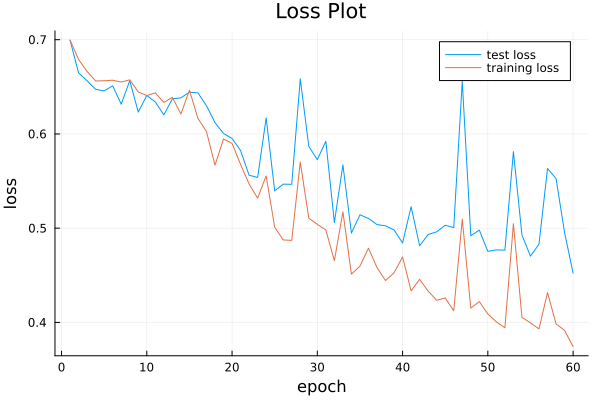
\includegraphics[width=0.4\linewidth]{loss_png_final_1_1.png}\hfill
	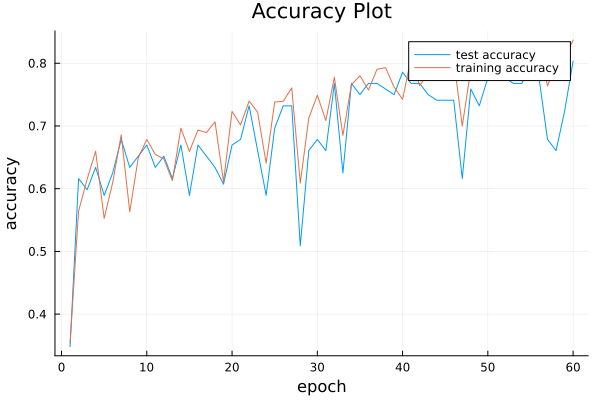
\includegraphics[width=0.4\linewidth]{accuracy_png_final_1_1.png}
	\\[\smallskipamount]
	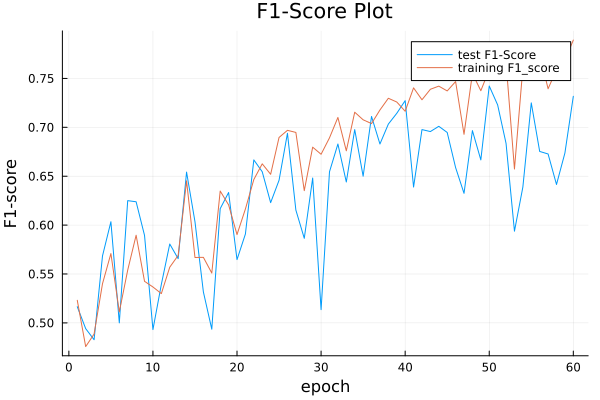
\includegraphics[width=0.4\linewidth]{f1_score_png_final_1_1.png}\hfill
	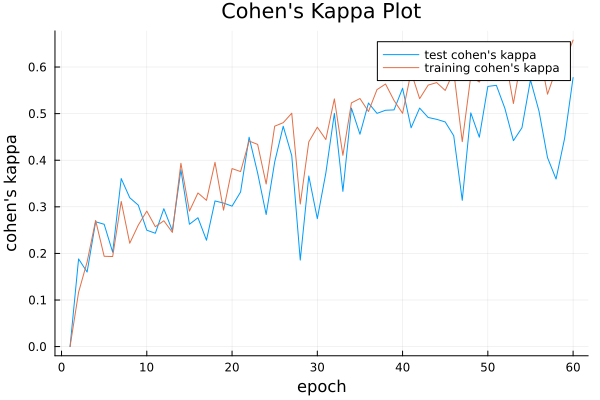
\includegraphics[width=0.4\linewidth]{cohens_kappa_png_final_1_1.png}
	\caption{model 1 (epochs: 60 loss: $50.3 \pm 4.5\% $ accuracy: $74.1 \pm6.3\%$ F1-score: $68.6 \pm3.5\%$  Cohen's kappa: $47.8\pm8.9$ )}
	\label{fig:model_1_60}
\end{figure}

\begin{figure}
	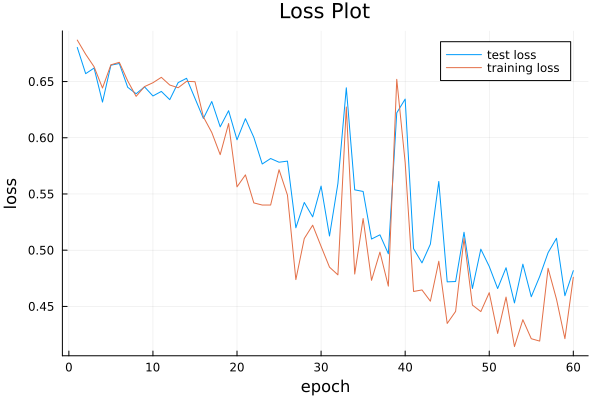
\includegraphics[width=0.4\linewidth]{loss_png_final_1_2.png}\hfill
	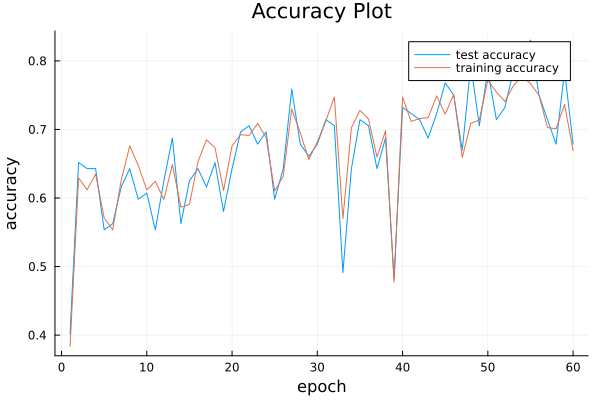
\includegraphics[width=0.4\linewidth]{accuracy_png_final_1_2.png}
	\\[\smallskipamount]
	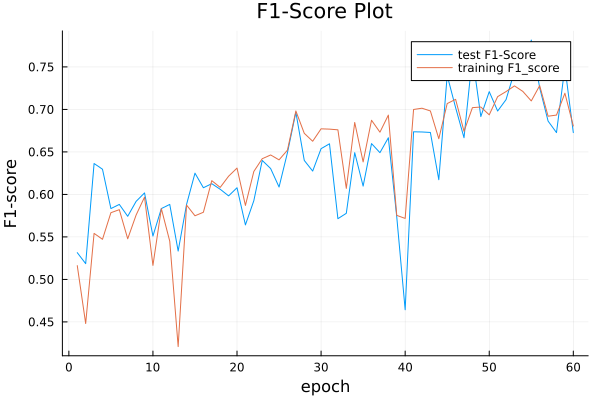
\includegraphics[width=0.4\linewidth]{f1_score_png_final_1_2.png}\hfill
	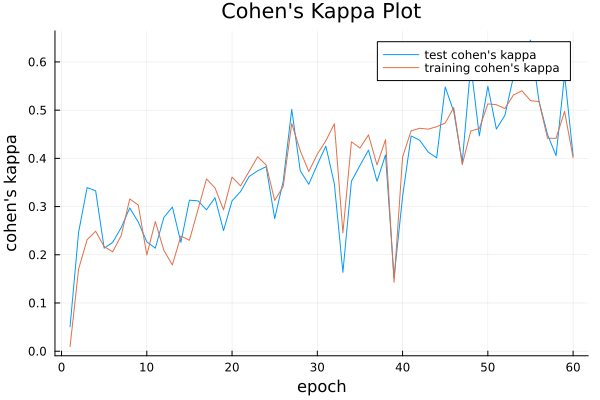
\includegraphics[width=0.4\linewidth]{cohens_kappa_png_final_1_2.png}
	\caption{model 2 (epochs: 60 loss: $48.1\pm2.1\% $ accuracy: $74\pm6.1\%$ F1-score: $71.5\pm4.5\%$  Cohen's kappa: $50\pm9.7$ )}
	\label{fig:model_2_60}
\end{figure}

\begin{figure}
	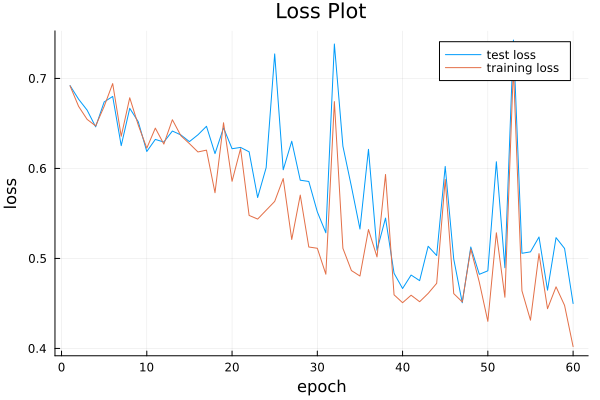
\includegraphics[width=0.4\linewidth]{loss_png_final_1_3.png}\hfill
	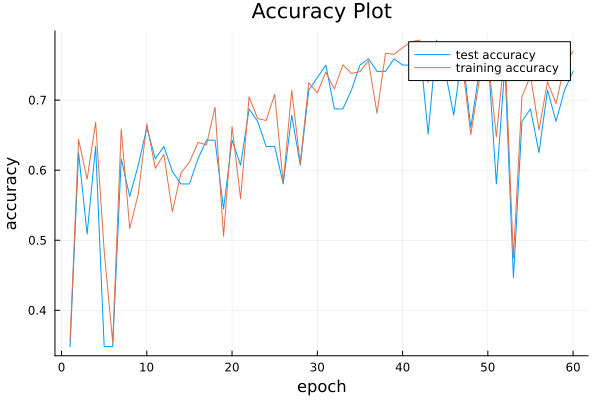
\includegraphics[width=0.4\linewidth]{accuracy_png_final_1_3.png}
	\\[\smallskipamount]
	\includegraphics[width=0.4\linewidth]{f1_score_png_final_1_3.png}\hfill
	\includegraphics[width=0.4\linewidth]{cohens_kappa_png_final_1_3.png}
	\caption{model 3(epochs:60 loss: $49.7\pm3.1\% $ accuracy: $69.2\pm4.1\%$ F1-score: $67.5\pm2.1\%$  Cohen's kappa: $42\pm5.5$ )}
	\label{fig:model_3_60}
\end{figure}

\begin{figure}
	\includegraphics[width=0.4\linewidth]{loss_png_final_1_4.png}\hfill
	\includegraphics[width=0.4\linewidth]{accuracy_png_final_1_4.png}
	\\[\smallskipamount]
	\includegraphics[width=0.4\linewidth]{f1_score_png_final_1_4.png}\hfill
	\includegraphics[width=0.4\linewidth]{cohens_kappa_png_final_1_4.png}
	\caption{model 4(epochs: 60 loss: $63.4\pm0.8\% $ accuracy: $62.2\pm3.1\%$ F1-score: $62.4\pm1.6\%$  Cohen's kappa: $31\pm4$ )}
	\label{fig:model_4_60}
\end{figure}

\begin{figure}
	\includegraphics[width=0.4\linewidth]{loss_png_final_2_1.png}\hfill
	\includegraphics[width=0.4\linewidth]{accuracy_png_final_2_1.png}
	\\[\smallskipamount]
	\includegraphics[width=0.4\linewidth]{f1_score_png_final_2_1.png}\hfill
	\includegraphics[width=0.4\linewidth]{cohens_kappa_png_final_2_1.png}
	\caption{model 5(epochs: 60 loss: $60.5\pm2.9\% $ accuracy: $67.8\pm2.8\%$ F1-score: $57.2\pm3.8\%$  Cohen's kappa: $32\pm2.6$ )}
	\label{fig:model_5_60}
\end{figure}

\begin{figure}
	\includegraphics[width=0.4\linewidth]{loss_png_final_2_2.png}\hfill
	\includegraphics[width=0.4\linewidth]{accuracy_png_final_2_2.png}
	\\[\smallskipamount]
	\includegraphics[width=0.4\linewidth]{f1_score_png_final_2_2.png}\hfill
	\includegraphics[width=0.4\linewidth]{cohens_kappa_png_final_2_2.png}
	\caption{model 6(epochs: 60 loss: $57\pm3\% $ accuracy: $68.5\pm8.8\%$ F1-score: $64.5\pm2.8\%$  Cohen's kappa: $39.1\pm10.7$ )}
	\label{fig:model_6_60}
\end{figure}

\begin{figure}[h]
	\includegraphics[width=0.4\linewidth]{loss_png_final_2_3.png}\hfill
	\includegraphics[width=0.4\linewidth]{accuracy_png_final_2_3.png}
	\\[\smallskipamount]
	\includegraphics[width=0.4\linewidth]{f1_score_png_final_2_3.png}\hfill
	\includegraphics[width=0.4\linewidth]{cohens_kappa_png_final_2_3.png}
	\caption{model 7 (epochs: 60 loss: $67.4\pm0.5\% $ accuracy: $53.3\pm2.4\%$ F1-score: $51.5\pm3.5\%$  Cohen's kappa: $12.8\pm4.6$ )}
	\label{fig:model_7_60}
\end{figure}

\begin{figure}[h]
	\includegraphics[width=0.4\linewidth]{loss_png_final_2_4.png}\hfill
	\includegraphics[width=0.4\linewidth]{accuracy_png_final_2_4.png}
	\\[\smallskipamount]
	\includegraphics[width=0.4\linewidth]{f1_score_png_final_2_4.png}\hfill
	\includegraphics[width=0.4\linewidth]{cohens_kappa_png_final_2_4.png}
	\caption{model 8 (epochs: 60 loss: $61\pm7.6\% $ accuracy: $73.5\pm1.9\%$ F1-score: $64.2\pm2.5\%$  Cohen's kappa: $43.3\pm3.2$ )}
	\label{fig:model_8_60}
\end{figure}

\begin{figure}[h]
	\includegraphics[width=0.4\linewidth]{loss_png_final_3_1.png}\hfill
	\includegraphics[width=0.4\linewidth]{accuracy_png_final_3_1.png}
	\\[\smallskipamount]
	\includegraphics[width=0.4\linewidth]{f1_score_png_final_3_1.png}\hfill
	\includegraphics[width=0.4\linewidth]{cohens_kappa_png_final_3_1.png}
	\caption{model 9 (epochs: 60 loss: $48.5\pm6.7\% $ accuracy: $71.3\pm7.9\%$ F1-score: $66\pm6\%$  Cohen's kappa: $43\pm10.9$ )}
	\label{fig:model_9_60}
\end{figure}

\begin{figure}[h]
	\includegraphics[width=0.4\linewidth]{loss_png_final_3_2.png}\hfill
	\includegraphics[width=0.4\linewidth]{accuracy_png_final_3_2.png}
	\\[\smallskipamount]
	\includegraphics[width=0.4\linewidth]{f1_score_png_final_3_2.png}\hfill
	\includegraphics[width=0.4\linewidth]{cohens_kappa_png_final_3_2.png}
	\caption{model 10 (epochs: 60 loss: $65.4\pm1.6\% $ accuracy: $59.7\pm9\%$ F1-score: $52.2\pm2.7\%$  Cohen's kappa: $19.8\pm10.1$ )}
	\label{fig:model_10_60}
\end{figure}

\begin{figure}[h]
	\includegraphics[width=0.4\linewidth]{loss_png_13_1.png}\hfill
	\includegraphics[width=0.4\linewidth]{accuracy_png_13_1.png}
	\\[\smallskipamount]
	\includegraphics[width=0.4\linewidth]{f1_score_png_13_1.png}\hfill
	\includegraphics[width=0.4\linewidth]{cohens_kappa_png_13_1.png}
	\caption{model 11 (epochs: 60 loss: $51.3\pm3.1\% $ accuracy: $73.4\pm4.3\%$ F1-score: $65.5\pm4.7\%$  Cohen's kappa: $44.6\pm6$ )}
	\label{fig:model_11_60}
\end{figure}

%\begin{figure}[h]
%	\includegraphics[width=0.4\linewidth]{loss_png_13_2_1.png}\hfill
%	\includegraphics[width=0.4\linewidth]{accuracy_png_13_2_1.png}
%	\\[\smallskipamount]
%	\includegraphics[width=0.4\linewidth]{f1_score_png_13_2_1.png}\hfill
%	\includegraphics[width=0.4\linewidth]{cohens_kappa_png_13_2_1.png}
%	\caption{model 12 (epochs: 60 loss: $69.2\pm8.9\% $ accuracy: $67.1\pm7.8\%$ F1-score: $61.9\pm2.2\%$  Cohen's kappa: $35.5\pm8.4$ )}
%\end{figure}

\clearpage

One of the tests includes to observe the impact of adding convolution layers to the end of the network. In model 1 (\ref{fig:model_1_60}) one additional layer is added. Its results are very similar but the training loss starts decreasing faster than the test loss. A similar phenomenon can be seen in the F1-Score and Cohen's kappa plot where the training plot slowly diverges from the test plot. In model 3 (\ref{fig:model_3_60}) with two additional convolution layers this effect does not appear but the accuracy is nearly 10 \% lower. The plots include some extreme outliers. In model 6 (\ref{fig:model_6_60}) padding was added to the layers. This increases the maximum accuracy to a similar level as without the additional convolutions but the amplitude of the oscillation increases as well.

Thereby it is concluded that adding new layers can quickly lead to a decrease in the networks performance. In contrast the addition of padding can reduce those effects. 
%Another test was switching convolutional layers by a custom Inception module. This model converges similar to the initial model but the amplitude of the oscillation is a bit stronger still the network also reaches accuracy values above 80 \% . model 4 switches the convolutional layers two and three by an inception modules.
%The loss of this network decreases slower than the initial model instead of a loss value around 0.4 we have a value close to 0.63. Also the accuracy does not converge at all constantly oscillating around 0.6. Just the F1-score and cohen's kappa sem to grow slowly but alson dont come close to the initial model. model 7 has an inception module in place of convolution three and four. In this model we can see the model slightly converging for the training data which has no effect on the test data.

\begin{figure}
%TODO: Inception modul that i use
\end{figure}
Another test is switching convolution layers by a custom inception module. Model 2 (\ref{fig:model_2_60}) switches the third convolution with an inception module. The performance of it is quite similar to our initial model. The loss plot decreases linear. The accuracy, F1-score and Cohen's kappa increase linear but the amplitude of the oscillation is a bit stronger. The network still reaches accuracy values above 80 \%.
In model 4 (\ref{fig:model_4_60}) and 7 (\ref{fig:model_7_60}) two convolution layers are switched with inception modules. The networks accuracy, F1-Score and Cohen's kappa stay constant while oscillating. The test loss of both models is also constant while the training loss slightly decreases. In model 7 (\ref{fig:model_7_60}) the network's performance of the test set is significantly worse than the training set.

These tests show that adding too many inception modules can be harmful to the performance of the network while adding one inception module might increase the network's performance in the long run. 

In model 5 (\ref{fig:model_5_60}) and 9(\ref{fig:model_9_60}) skip connections are attached to the network. The loss of model 5 (\ref{fig:model_5_60}) decreases linear and the accuracy and Cohen's kappa increase linear but the F1-score increases slightly. This model does not perform as well as the initial network but still seems to be growing. Model 9 (\ref{fig:model_9_60}) performs better than the initial network. Its accuracy, F1-score and Cohen's kappa are similar but the loss is 0.05 lower than the loss of the initial network. 
This means that the addition of skip connections can be beneficial to the overall performance of the network.

In model 8 (\ref{fig:model_8_60}) the number of filters of some convolution layers is increased. The training graphs look similar to the ones of the initial networks. The loss of the test set is similar to the training loss until epoch 35. Afterwards it stops decreasing, the gradient of accuracy, F1-Score and Cohen's kappa also decreases significantly. This model shows that even a slight increase of the network's parameters can have a major impact.

Model 10 (\ref{fig:model_10_60}) removes the max pooling layers and instead uses stride to quickly reduce the size of the input image. This was preformed to get a understanding of the importance the max pooling layer type. Looking at the results it can be observed that the accuracy plot oscillates strongly and barely reaches a value above 80\%. Furthermore, the loss plot shows strong oscillation and the training and the test plot seem to diverge.

In model 11 (\ref{fig:model_11_60}) the effect of multiple dense layers on the networks performance is evaluated. The loss plots are oscillating and seem to diverge. Even though a lower accuracy is reached, it does not reach the 80 \% mark. The F1-score and Cohen's kappa graphs reach high values while oscillating significantly and showing signs of divergence.

In conclusion it can be stated that the addition of parameters to the network needs to be handled with care since even the addition of a few layers / kernels can lead to overfitting. In some cases, it occurs that the network does not converge even when reducing the learning rate.
After these test a combination of certain methods is applied and the effect on the network's performance is evaluated. 

\begin{table}
	\begin{tabular}{cccccc}
		\toprule
		\multicolumn{2}{c}{model 12} &\multicolumn{2}{c}{model 13} & \multicolumn{2}{c}{model 14} \\ 
		Layer & Output &Layer & Output &Layer & Output\\
		\cmidrule(l){1-2} \cmidrule(l){3-4}\cmidrule(l){5-6}
		Input&(,512,512,1)&Input&(,512,512,1)&Input&(,512,512,1)\\
		\cmidrule(l){1-2} \cmidrule(l){3-4}\cmidrule(l){5-6}
		Conv2D& (,511,511,16) &Conv2D	& (,511,511,16)&Conv2D	& (,511,511,16)\\
		\cmidrule(l){1-2} \cmidrule(l){3-4}\cmidrule(l){5-6}
		MaxPool&(,256,256,16)&MaxPool&(,256,256,16)&MaxPool&(,256,256,16)\\
		\cmidrule(l){1-2} \cmidrule(l){3-4}\cmidrule(l){5-6}
		Conv2D&(,255,255,16)&Conv2D&(,255,255,16)&Conv2D&(,255,255,16)\\
		\cmidrule(l){1-2} \cmidrule(l){3-4}\cmidrule(l){5-6}
		MaxPool&(,128,128,16)&MaxPool&(,128,128,16)&MaxPool&(,128,128,16)\\
		\cmidrule(l){1-2} \cmidrule(l){3-4}\cmidrule(l){5-6}
		Inception&(,128,128,16)&Conv2D&(,127,127,16)&Inception&(,128,128,16)\\
		\cmidrule(l){1-2} \cmidrule(l){3-4}\cmidrule(l){5-6}
		MaxPool&(,64,64,16)&MaxPool&(,64,64,16)&MaxPool&(,64,64,16)\\
		\cmidrule(l){1-2} \cmidrule(l){3-4}\cmidrule(l){5-6}
		Conv2D&(,63,63,16)&Conv2D&(,63,63,16)&Conv2D&(,63,63,16)\\
		\cmidrule(l){1-2} \cmidrule(l){3-4}\cmidrule(l){5-6}
		MaxPool&(,32,32,16)&MaxPool&(,32,32,16)&MaxPool&(,32,32,16)\\
		\cmidrule(l){1-2} \cmidrule(l){3-4}\cmidrule(l){5-6}
		Conv2D&(,32,32,16)&Skip2&(,32,32,16)&Skip2&(,32,32,16)\\
		\cmidrule(l){1-2} \cmidrule(l){3-4}\cmidrule(l){5-6}
		Conv2D&(,32,32,16)&GAP&(,16)&GAP&(,16)\\
		\cmidrule(l){1-2} \cmidrule(l){3-4}\cmidrule(l){5-6}
		Conv2D&(,32,32,16)&Dense&(,1)&Dense&(,1)\\
		\cmidrule(l){1-2}
		GAP&(,16)&&&&\\
		\cmidrule(l){1-2}
		Dense&(,1)&&&&\\
		
		%Todo GAP needs to be defined somewhere	 	
	\end{tabular}
	\caption{Skip2: A skip connection with two 3x3 Convolutions}
	
\end{table}

\begin{figure}[h]
	\includegraphics[width=0.4\linewidth]{loss_png_12_1.png}\hfill
	\includegraphics[width=0.4\linewidth]{accuracy_png_12_1.png}
	\\[\smallskipamount]
	\includegraphics[width=0.4\linewidth]{f1_score_png_12_1.png}\hfill
	\includegraphics[width=0.4\linewidth]{cohens_kappa_png_12_1.png}
	\caption{model 12 (epochs: 60 loss: $\pm50.4\%5.7 $ accuracy: $73.7\pm7.1\%$ F1-score: $68.3\pm6.8\%$  Cohen's kappa: $47.3\pm10.7$ )}
	\label{fig:model_12_200}
\end{figure}



\begin{figure}
	\includegraphics[width=0.4\linewidth]{loss_png_13_3.png}\hfill
	\includegraphics[width=0.4\linewidth]{accuracy_png_13_3.png}
	\\[\smallskipamount]
	\includegraphics[width=0.4\linewidth]{f1_score_png_13_3.png}\hfill
	\includegraphics[width=0.4\linewidth]{cohens_kappa_png_13_3.png}
	\caption{model 9 (epochs: 200 loss: $61.7\pm12.9\% $ accuracy: $72\pm3.5\%$ F1-score: $65.5\pm3.1\%$  Cohen's kappa: $42.9\pm4.7$ )}
	\label{fig:model_9_200}
\end{figure}


\begin{figure}
	%14_3
	\includegraphics[width=0.4\linewidth]{loss_png_final_run_6_1.png}\hfill
	\includegraphics[width=0.4\linewidth]{accuracy_png_final_run_6_1.png}
	\\[\smallskipamount]
	\includegraphics[width=0.4\linewidth]{f1_score_png_final_run_6_1.png}\hfill
	\includegraphics[width=0.4\linewidth]{cohens_kappa_png_final_run_6_1.png}
	\caption{model 13 (epochs: 200 loss: $40.7\pm6.8\% $ accuracy: $82.2\pm1.1\%$ F1-score: $75.3\pm2.8\%$  Cohen's kappa: $61.5\pm2.6$ )}
	\label{fig:model_13_200}
\end{figure}

\begin{figure}
	\includegraphics[width=0.4\linewidth]{loss_png_14_4.png}\hfill
	\includegraphics[width=0.4\linewidth]{accuracy_png_14_4.png}
	\\[\smallskipamount]
	\includegraphics[width=0.4\linewidth]{f1_score_png_14_4.png}\hfill
	\includegraphics[width=0.4\linewidth]{cohens_kappa_png_14_4.png}
	\caption{model 14 (epochs: 200 loss: $52.8\pm2.3\% $ accuracy: $79.8\pm2.4\%$ F1-score: $68.6\pm3.5\%$  Cohen's kappa: $53.9\pm4.9$ )}
	\label{fig:model_14_200}
\end{figure}
	\clearpage 
	
During testing of the final models, the model is trialed for 60 epochs and if it performes well, it is trained for 200 epochs. The only model which didn't perform well enough for trialing it for 200 epochs was model 12 (\ref{fig:model_12_200}). This model stayed similar for the 40 epochs and then made a huge jump but still only achieved a max accuracy of around 70 percent which didn't seem to be able to contend the initial model. 

The models that are trained for 200 epochs always achieved similar peak performances compared to the initial network. In model 9 (\ref{fig:model_9_200}) shortly after reaching its peak performance, the training and test performance graphs start to diverge. While the performance of the training set becomes better, the test set performance slightly decreases. This is interpreted as overfitting of the network due to a lack of training data.

The only model that reaches a higher peak accuracy then the initial network is model 13 (\ref{fig:model_13_200}) with 85.6 \%. Its performance is significantly more stable as its oscillation is minor.

model 14 (\ref{fig:model_14_200}) on the other hand has a very slow performance growth which reaches its peak around epoch 200. This indicates that this model might outperform the initial model. However, when training the same network for 300 epochs the result was different than expected with the accuracy only reaching around 71\% after 290 epochs even after running this simulation multiple times its results didn't change. The good results when training for 200 epochs are consequently contributed to a lucky choice of the initial parameters.
%\chapter{Experimental Setup}

\begin{figure}[h]
	\centering
	\begin{minipage}[t]{.45\linewidth}
		\centering
		\includegraphics[width = \textwidth]{accuracy_per_scan_type_final_run_6_2.png}%
		\captionsetup{width=\textwidth}
		\caption{accuracy of scan type 1-5 of the initial model \\ (Type 1 accuracy: $94.4\pm5.1\%$, Type 2 accuracy: $97.9\pm2.6\%$, Type 3 accuracy: $72.9\pm6.6\%$, Type 4 accuracy: $70.7\pm6.2\%$, Type 5 accuracy: $99.7\pm0.6\%$ )}
		\label{fig:run_6_2_all_accs}
		
	\end{minipage}
	\hfill
	\begin{minipage}[t]{.45\linewidth}
		\centering
		\includegraphics[width = \textwidth]{accuracy_per_scan_type_final_run_6_1.png}%
		\caption{accuracy of scan type 1-5 of model 13 \\(Type 1 accuracy:$99.4\pm0.9\%$, Type 2 accuracy: $97.6\pm2.1\%$, Type 3 accuracy: $72.2\pm9.4\%$, Type 4 accuracy: $75.9\pm9.2\%$, Type 5 accuracy: $92.3\pm12.1\%$) }
		\label{fig:run_6_1_all_accs}
	\end{minipage}
\end{figure}

Subsequently, the accuracy of the initial model and model 13 are analyzed for every single scan type. This figure is chosen to visualize the difference in accuracy between the different scan types. The networks especially perform well on type 1,2 and 5 scans which achieve a mean accuracy of over 90\% . If compared to type 3 and 4 scans, they only reach mean accuracy values around 70-76 \% which is a significantly lower.

\chapter{Discussion}

The object of this thesis was to replicate the results of \citet{Walle2023} and try to validate its findings for data generated by the Scanco XtremeCT I. Its model can be used to support operators in determining the severity of motion in radius and tibia scans while reducing the operator's bias. In the field of medicine it is desirable to minimize false assessments. Therefore, a high accuracy of the model is beneficial. In these cases this would lead to some patients not needing another re-scan which would reduce the radiation the patient is exposed to. Based on the findings  of \citet{Walle2023} a more sophisticated network is developed while sticking to a general CNN approach. 

When trying to replicate the results of \citet{Walle2023}, the impact of different augmentation techniques on the data set was evaluated.Furthermore, the impact of static and dynamic learning rate on the training process was reviewed. On one hand  traditional augmentation techniques were implemented. On the other hand the work of other researchers in similar fields was taken into consideration. One method used by \citet{Zhang2020} is to rotate the images by 1-5$^{\circ}$ which seemed to be promising, since the use of 1-360$^{\circ}$ rotation did not achieve satisfying results. This method returned a high accuracy but after its peak around epoch 50 the test and training accuracy started to diverge which might be due to the network overfitting on the data. The most promising results for this network is by a $ n \cdot 90^{\circ} $ rotation with n $\in$ {0-3}$\mathbb{N}$, Gaussian noise, image snippets, horizontal and vertical flipping. 

Additionally, different learning rates for optimizers of the Adam family were implemented. The results of these tests show the superiority of basic Adam without any learning rate decay. Even when training the network with a combination of the best augmentation technique and optimizer we still didn't get close to the performance of \citet{Walle2023}. In the research following this assessment the same augmentation and optimizers are used. In some cases, especially when using larger networks, the learning rate had to be reduced to 0.0001 instead of 0.001 which needs to be considered when building on this research.


The results of this thesis are difficult to compare to the results of the initial paper since its scans where generated by the XtremeCT II. \citet{Walle2023} This scanner has a scan time of 120 seconds which is less than the XtremeCT I which has a scan time of at least 168 seconds. \citet{Tran2019} The smaller scan time reduces the risk of a patient moving and therefore the distribution of the severity level is different compared to the data used in this paper. This leads to more type 1 and 2 scans whilst reducing type 3 and 4 scans. While there is no information in the paper \citet{Walle2023} about this distribution, it is suspected that this influences the overall accuracy. Looking at the performance of our network for the different severity types, the network performes well on type 1,2 and 5 scans with mean accuracy values of over 90\% while type 3 and 4 scans have a significantly lower accuracy of around 70-76\%. This supports the assumption that the different distribution of scan types caused by the newer scanner improves the accuracy of the network significantly. This theory should be validated by using data generated by the XtremeCT II scanner. Furthermore, type 1,2 and 5 scans often reach 100 percent accuracy which is a sign that the network overfits on those data types. 

Another reason why our network might have performed worse is that the initial paper includes a visual examination of the network by using the Grad-CAM method. The Grad-CAM method is used to interpret the network's decisions. This method wasn't applicable in this thesis due to the lack of healthcare professionals to interpret if the network looks at the correct regions to determine the severity of scans. Also, Grad-CAM is not implemented. Since the implementation of it would have exceeded the scope of this work, it is excluded. 

Based on the findings of the replication of \citet{Walle2023}, the object has been to find a model that performs better on the given data. This was done by adding additional layers, kernels or switching layers with skip connections and inception modules. Sometimes, due to a lack of training data even small changes on the networks structure had major effects on the network performance. Most of the models showed no real improvement to the initial network. Most of the networks seemed to struggle with the amount of given data or did not show any significant difference in performance to have a major effect on the results. Only one model outperformed the initial model (loss: $40.7\pm6.8\% $ accuracy: $82.2\pm1.1\%$ F1-score: $75.3\pm2.8\%$  Cohen's kappa: $61.5\pm2.6$ ) with the highest recorded accuracy being 85.62\%. This is 1.13 percent higher than the highest accuracy of the initial network. Additionally, it seems to be more stabled since it has less oscillation. 
%TODO: hier muss noch hin das die verschiedenen typen auch ähnlich wie in dem initialen model erkannt werden.

Even though not all of the layer performed as well, the addition of inception and skip connections seemed to have a positive effect on the network's performance. One major contributor to the networks not reaching higher performance is attributed to the size of the training set. To prove this theory, testing on a larger data set is necessary. 

\chapter{Conclusion}
As a conclusion it can be said that the network described in \citet{Walle2023} is a good fit for the amount of training data used. Small data sets often bring the issue with them, that even networks with a few layers can be prone to overfitting. This can be seen in this paper. Even the addition of a few more parameters leads the network to overfit or result in significantly worse results. This is not as visible when training for only 60 epochs, but when training for 200 epochs it becomes obvious.

It is hard to compare our findings with the results of \citet{Walle2023} since the paper used scans of the XtremeCT II. The network achieve significantly lower performances on the used data from the XtremeCT I scanner. When looking at the performance of the different scan types, the network has a mean accuracy of over 90\% for type 1,2 and 5 scans and only 70-76\% mean accuracy for type 3 and 4 scans. Since the XtremeCT I has a longer scan time, scans are more likely to contain type 3 and 4 motion artifacts. The reduction of those scan types, which might be possible by using the XtremeCT II, might lead our network to achieve better performances. To prove this theory a test on XtremeCT II scans is recommend. 

By analyzing the performance of operators on the data it becomes apparent that the main issue is the detection of type 3 and 4 scans. Therefore, an overall high accuracy won't support the operators in their work if they can't rely on the network's performance for detecting type 3 and 4 scans. A network which is only trained on this type of data (type 3 and 4 scans) might be able to achieve higher performances and consistently be able to reduce the human bias when its influence is the strongest. 

Even with the small amount of data it was possible to achieve a small increase in the peak accuracy and stability of the network. This was accomplished by switching the fifth convolution layer with a skip connection containing two convolution layers. In other tests the training and test graphs often started to diverge which indicates that the networks overfitted. It still showed signs that the addition of inception layers and skip connections might be able to benefit the network when trained on a bigger data set. Therefore, it is proposed to repeat the tests on a larger data set to evaluate which impact this changes have on the network's performance. 


%should develope a network that tries to focus on detecting type 3 and 4 scans correctly since this is the major obstacle for operators 
%TODO: this chapter needs to be written and finsihed

\bibliographystyle{plainnat}
%\bibliographystyle{IEEEtranN}
%\bibliographystyle{unsrt} %unsrt abbrv
\bibliography{Bibliography}

\end{document}
